\section{约束优化最优性条件}
\[
    \begin{array}{ll}
        \min & f(\boldsymbol{x})\\
        \mathrm{s.t.} & \boldsymbol{x}\in\Omega
    \end{array}
\]
\[
    \Omega=\{\boldsymbol{x}\in\mathbb{R}^{n}|c_{i}(\boldsymbol{x})=0,i\in\mathcal{E};c_{i}(\boldsymbol{x})\geqslant 0, i\in\mathcal{I}\},
\]
\begin{figure}[htbp]
    \centering
    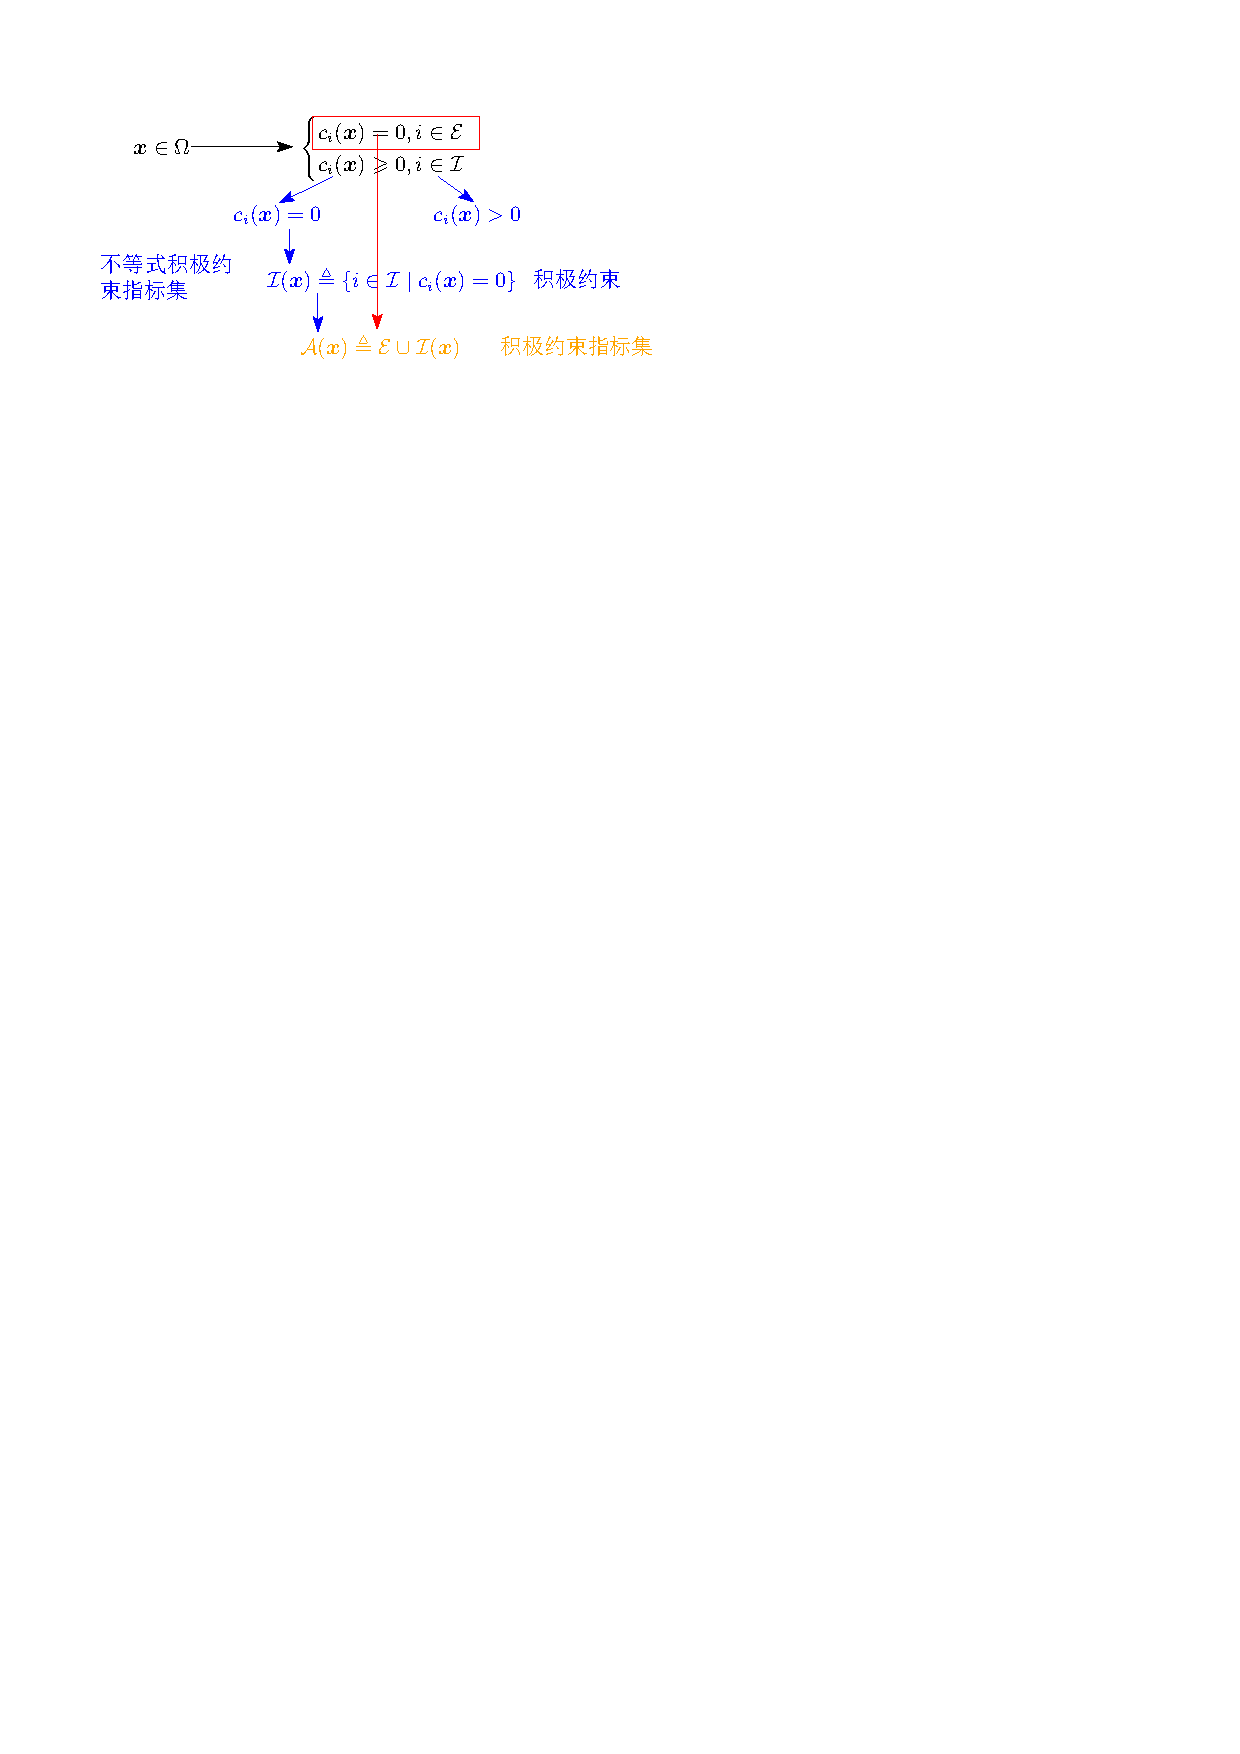
\includegraphics{image/积极约束指标集.pdf}
\end{figure}
\begin{definition}[可行方向]
    设设$\boldsymbol{x}\in \Omega$对$\boldsymbol{d}\in\mathbb{R}^{n}$若存在$\delta>0$,使对任意的$\alpha\in[0,\delta]$都有$\boldsymbol{x}+\alpha\boldsymbol{d}$则称$\boldsymbol{d}$为约束优化问题在$\boldsymbol{x}$点的可行方向.
\end{definition}
\begin{note}
    有的可行域没有可行方向,如$\Omega=\{\boldsymbol{x}\in \mathbb{R}^n\mid\boldsymbol{x}^{\mathrm{T}}\boldsymbol{x}=1\}$
    \begin{figure}[H]
        \centering
        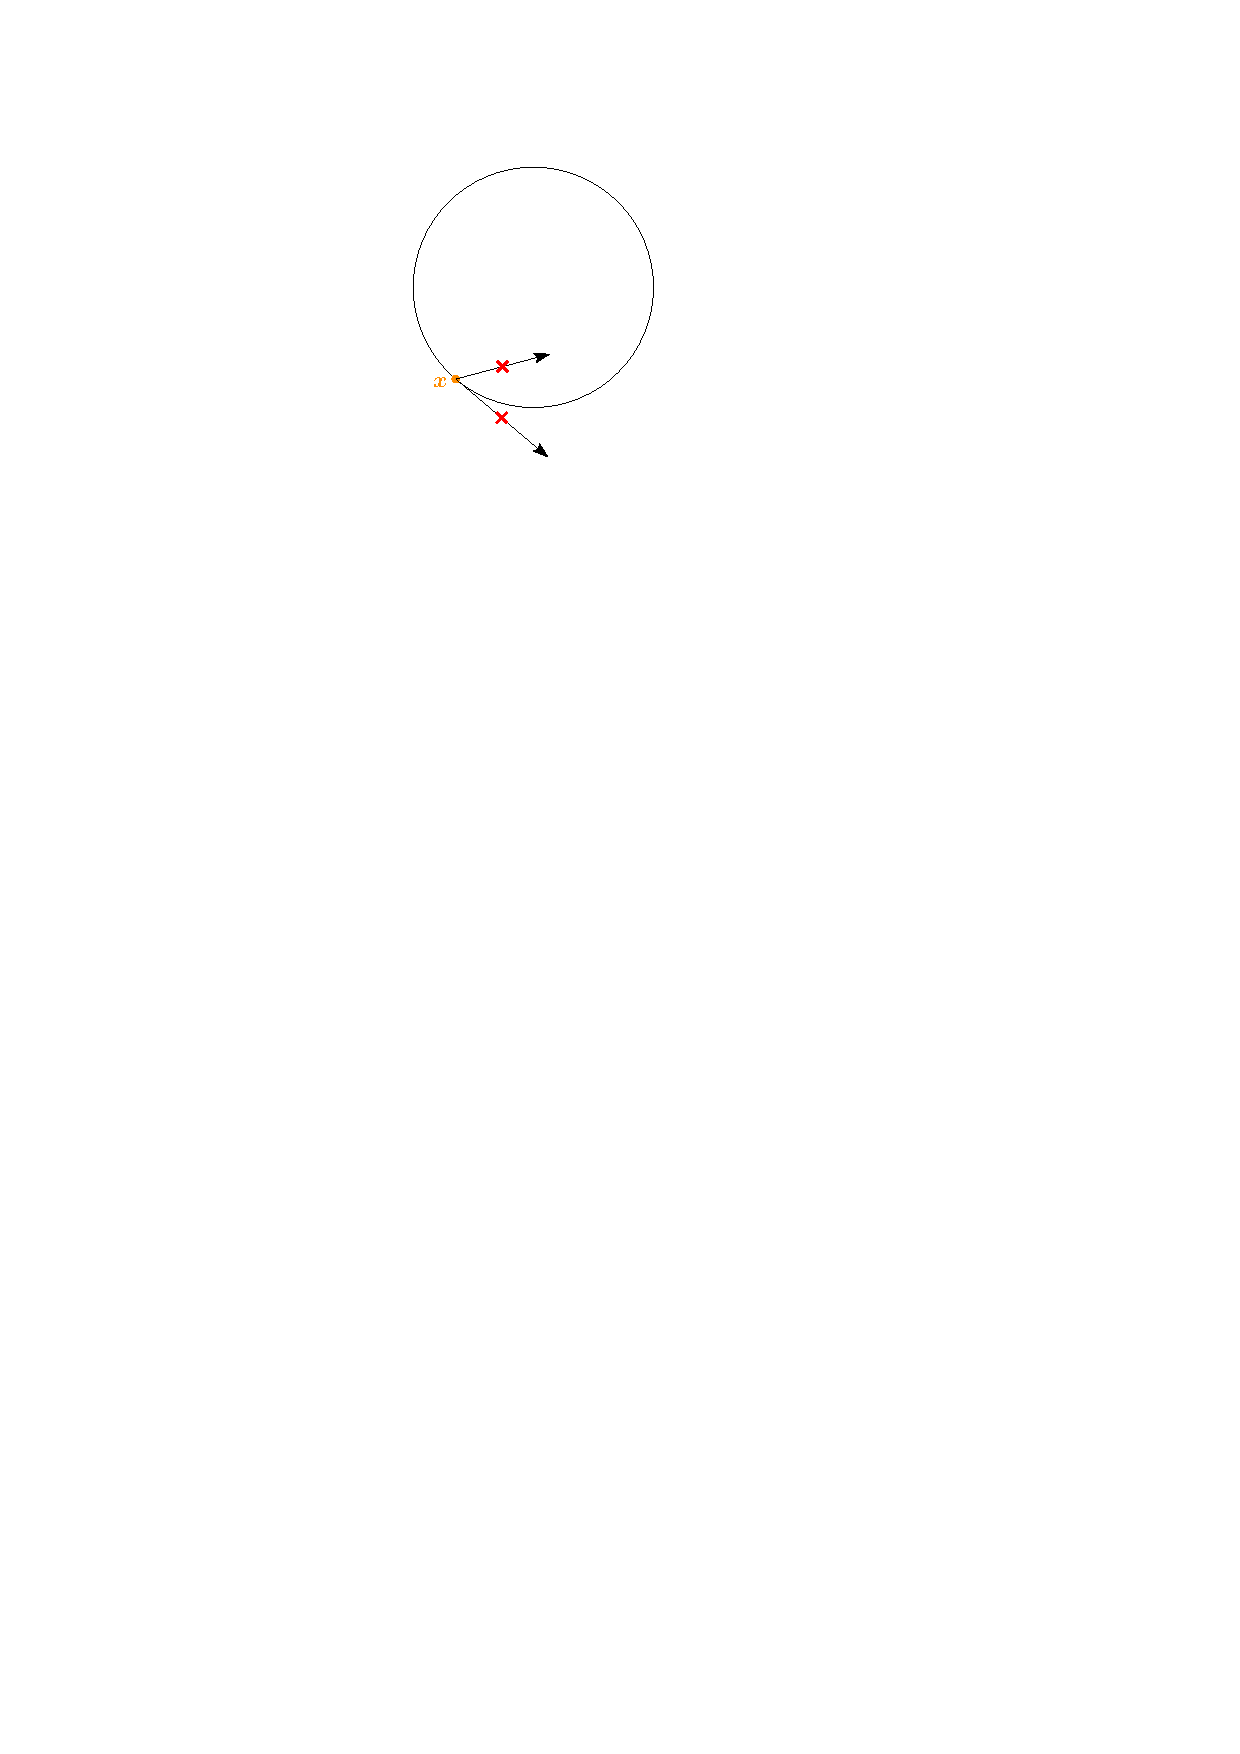
\includegraphics{image/无可行方向的可行域.pdf}
    \end{figure}
\end{note}
\begin{corollary}
    若$\boldsymbol{d}$为约束优化问题在$\boldsymbol{x}\in \Omega$点的可行方向, 则(必要条件)
    \[
        \colorbox{cyan!50}{$\nabla c_i(\boldsymbol{x})^\mathrm{T}\boldsymbol{d}=0,\quad\forall i\in\mathcal{E};$}\quad \colorbox{red!50}{$\nabla c_i(\boldsymbol{x})^\mathrm{T}\boldsymbol{d}\geqslant 0,\quad\forall i \in\mathcal{I}(\boldsymbol{x}).$}
    \]
    \colorbox{cyan!50}{第一个条件是确保垂直};\colorbox{red!50}{第二个条件是确保边界点的下一步在可行域内}

    \textcolor{red}{特别提醒:上述条件不是充分的,除非约束函数是线性的。}
\end{corollary}
\begin{theorem}[可行下降方向]
    若$\boldsymbol{d}$为$\boldsymbol{x}\in\Omega$点的可行方向, 同时还是目标函数在该点的下降方向,则称其为目标函数在该点的可行下降方向。

    最优值点不存在可行下降方向
\end{theorem}
\begin{theorem}
    若约束优化问题的可行域为非空闭凸集,则最优解$\boldsymbol{x}^*$为约束优化问题的\textcolor{red}{稳定点},即满足
    \[
        \langle\nabla f(\boldsymbol{x}^{*}),{\boldsymbol{x}-\boldsymbol{x}^{*}}\rangle\geqslant0,\quad\forall\boldsymbol{x}\in\Omega.
    \]
    \begin{figure}[htbp]
        \centering
        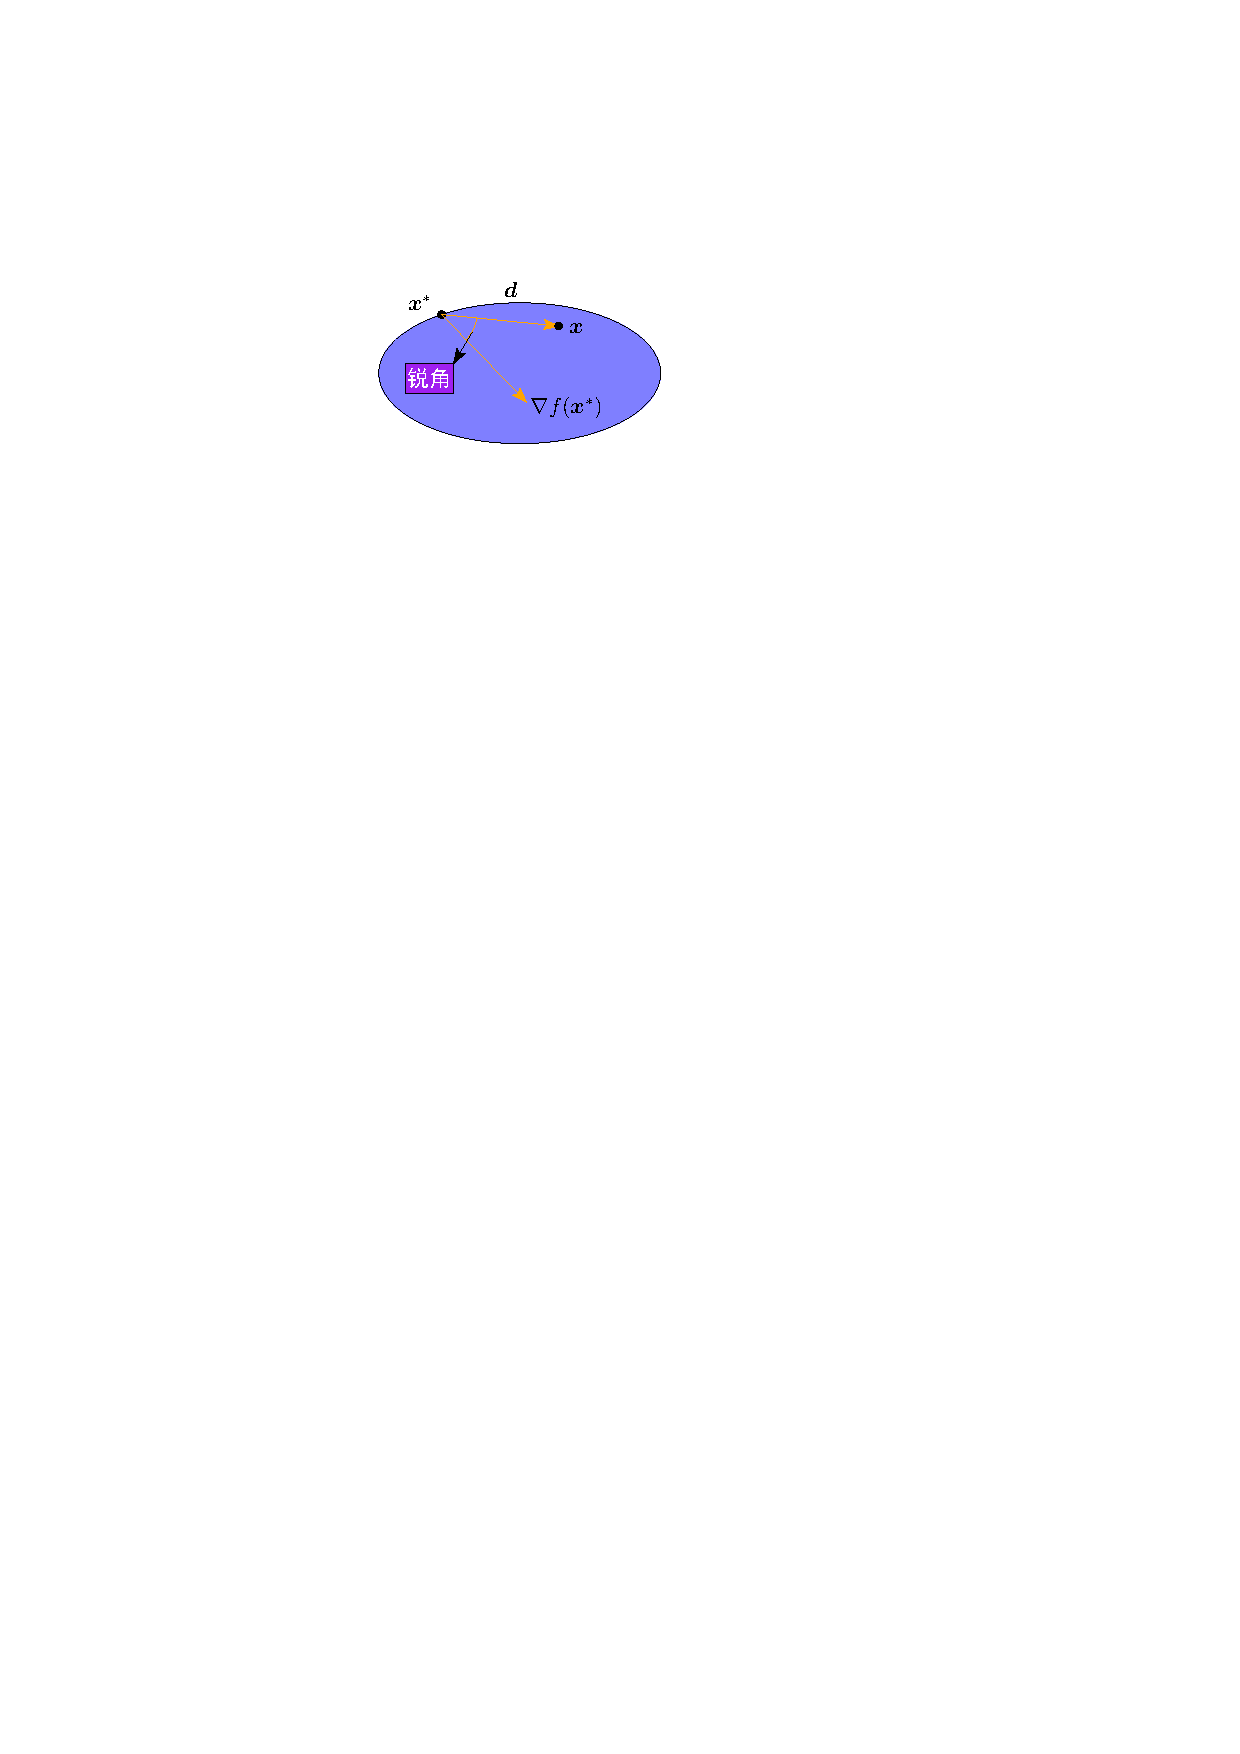
\includegraphics{image/约束优化问题的稳定点.pdf}
    \end{figure}
\end{theorem}
\subsection{等式优化最优化条件}
\begin{example}
    设$\boldsymbol{a}_1,\boldsymbol{a}_2,\cdots,\boldsymbol{a}_m\in\mathbb{R}^n$满足$\sum\limits_{i = 1}^{m}\boldsymbol{a}_{i}\neq \boldsymbol{0}$求解优化问题\Stars{5}{}
    \[
        \min\{\sum_{i=1}^{m}\|\boldsymbol{x}-\boldsymbol{a}_{i}\|^{2}\mid\boldsymbol{x}^{\mathrm{T}}\boldsymbol{x}=1\}
    \]
    \begin{solution}
        令
        \[
            \begin{aligned}
                L(\boldsymbol{x},\lambda)&=\|\boldsymbol{x}-\boldsymbol{a}_{i}\|^{2}-\lambda(\boldsymbol{x}^{\mathrm{T}}\boldsymbol{x}-1)\\
                &=\sum_{i=1}^{m}\sum_{j=1}^{n}\left( \boldsymbol{x}_j-(\boldsymbol{a}_{i})_{j} \right)^2-\lambda\left( \sum_{j = 1}^{n}\boldsymbol{x}_j^2-1\right)
            \end{aligned}
        \]
        对$x_k$求偏导,得到
        \[
            \dfrac{\partial L}{\partial x_{k}} = \sum_{i = 1}^{m}2(x_{k}-(\boldsymbol{a}_{i})_{k})-\lambda\cdot 2 x_{k}
        \]
        故而有
        \[
            \nabla_{x}L = \begin{pmatrix}
                \sum_{i = 1}^{m}2(x_{1}-(\boldsymbol{a}_{i})_{1})-\lambda 2x_{1}\\
                \sum_{i = 1}^{m}2(x_{2}-(\boldsymbol{a}_{i})_{2})-\lambda 2x_{2}\\
                \vdots\\
                \sum_{i = 1}^{m}2(x_{n}-(\boldsymbol{a}_{i})_{n})-\lambda 2x_{n}\\
            \end{pmatrix} 
        \]
        所以,有
        \[
            \begin{cases}
                \sum\limits_{i = 1}^{m}2(\boldsymbol{x-\boldsymbol{a}_{i}}) = 2\lambda\boldsymbol{x}\\
                \boldsymbol{x}^{\mathrm{T}}\boldsymbol{x}=1
            \end{cases}
        \]
        设方程的解为$\boldsymbol{x}^*$,则$\boldsymbol{x}^*$与$\sum\limits_{i = 1}^{m}\boldsymbol{a}_i$同向或者反向。

        若$\sum\limits_{i = 1}^{m}\boldsymbol{a}_i \neq \boldsymbol{0}$,则
        \[
            \boldsymbol{x}^*=\dfrac{\sum_{i=1}^m\boldsymbol{a}_i}{\|\sum_{i=1}^m\boldsymbol{a}_i\|}
        \]
        相应地,最优值为
        \[
            \begin{aligned}
                f(\boldsymbol{x}^*) &= \sum_{i=1}^{m}\|\boldsymbol{x}^*-\boldsymbol{a}_{i}\|^{2} \\
                & = \sum_{i=1}^{m}\left< \boldsymbol{x}^*-\boldsymbol{a}_{i},\boldsymbol{x}^*-\boldsymbol{a}_{i} \right>\\
                & =\sum_{i=1}^{m}\|\boldsymbol{x}^*\|^2-2\left<\dfrac{\sum_{i=1}^m\boldsymbol{a}_i}{{\|\sum_{i=1}^m\boldsymbol{a}_i\|}},\sum_{i=1}^m\boldsymbol{a}_i\right>+\sum_{i=1}^m\|\boldsymbol{a}_i\|^2\\
                &=m-2\|\sum_{i=1}^m\boldsymbol{a}_i\|+\sum_{i=1}^m\|\boldsymbol{a}_i\|^2
            \end{aligned}
        \]
    \end{solution}
\end{example}
\subsubsection{不等式优化约束条件}
\[
    \begin{array}{ll}
        \min&f(\boldsymbol{x})\\
        \mathrm{s.t.}&\boldsymbol{a}_{i}^{\mathrm{T}}\boldsymbol{x}+b_{i}=0,i\in\mathcal{E}\\
        &\boldsymbol{a}_{i}^{\mathrm{T}}\boldsymbol{x}+b_{i}\geqslant0,i\in\mathcal{I}
    \end{array}
\]
\begin{theorem}[完整KKT条件]
    \[
        \left\{
            \begin{aligned}
                &\nabla f(\boldsymbol{x}^{*})=\sum_{i\in\mathcal{E}\cup\mathcal{I}}\lambda_{i}^{*}\nabla c_{i}(\boldsymbol{x}^{*}),\\
                &\lambda_{i}^{*}\geqslant 0,\,c_{i}(\boldsymbol{x}^{*})\geqslant 0,\,\lambda_{i}^{*}c_{i}(\boldsymbol{x}^{*})=0,\,i\in\mathcal{I},\\
                &c_{i}\big(\boldsymbol{x}^{*}\big)=0,\,i\in\mathcal{E}.
            \end{aligned}
        \right.
    \]
\end{theorem}
\subsection{鞍点与凸规划}
\begin{definition}[函数的鞍点]
    梯度零点,但既不是最大值点、也不是最小值点
\end{definition}
% \begin{example}
%     证明以下问题为凸规划问题\Stars{2}{}
%     \[
%         \min 
%     \]
% \end{example}
\subsection{约束优化对偶}
\subsubsection{Lagrange对偶}
原问题:
\[
    \begin{array}{lcr}
        \min f(\boldsymbol{x}) & \Longrightarrow & \min f(\boldsymbol{x}) \\
        \operatorname{s.t.} c_{i}(\boldsymbol{x}) = 0,\,i\in \mathcal{E} & \Longrightarrow & \boldsymbol{H}(\boldsymbol{x}) = \boldsymbol{0} \\
        \operatorname{s.t.} c_{i}(\boldsymbol{x}) \geqslant 0,\,i\in \mathcal{I} & \Longrightarrow & \boldsymbol{G}(\boldsymbol{x}) \geqslant \boldsymbol{0}
    \end{array}
\]
Lagrange函数
\[
    \min_{\boldsymbol{x}\in\mathbb{R}^n}\max_{\boldsymbol{u}\geqslant \boldsymbol{0},\boldsymbol{v}}L(\boldsymbol{x},\boldsymbol{u},\boldsymbol{v}) = f(\boldsymbol{x})-\boldsymbol{G}(\boldsymbol{x})^{\mathrm{T}}\boldsymbol{u}-\boldsymbol{H}(\boldsymbol{x})^{\mathrm{T}}\boldsymbol{v},\,\boldsymbol{x}\in\mathbb{R}^n,\,\boldsymbol{u}\in \mathbb{R}_{+}^{|\mathcal{I}|},\,\boldsymbol{v}\in\mathbb{R}^{|\mathcal{E}|}
\]
对偶问题:
\[
    \max_{\boldsymbol{u}\geqslant \boldsymbol{0},\boldsymbol{v}}\min_{\boldsymbol{x}\in\mathbb{R}^n}L(\boldsymbol{x},\boldsymbol{u},\boldsymbol{v}) = \max_{\boldsymbol{u}\geqslant \boldsymbol{0},\boldsymbol{v}} \theta(\boldsymbol{u},\boldsymbol{v})
\]
\begin{example}
    线性规划的对偶\Stars{5}{}
    \[
        \begin{array}{rl}
            \min & \boldsymbol{c}^\mathrm{T}\boldsymbol{x}\\
            \mathrm{s.t.} & \boldsymbol{Ax}=\boldsymbol{b}\\
            & \boldsymbol{x}\geqslant\boldsymbol{0}
        \end{array}
    \]
    对偶
    \[
        \max_{\boldsymbol{u}\geq0,\boldsymbol{v}}\min_{\boldsymbol{x}\in \mathbb{R}^n}L(\boldsymbol{x},\boldsymbol{u},\boldsymbol{v})
    \]
    \[
        \begin{aligned}
            L(\boldsymbol{x};\boldsymbol{u},\boldsymbol{v})&=\boldsymbol{c}^\mathrm{T}\boldsymbol{x}-\boldsymbol{u}^\mathrm{T}\boldsymbol{x}-\boldsymbol{v}^\mathrm{T}(\boldsymbol{A}\boldsymbol{x}-\boldsymbol{b})\\
            &=\left(\boldsymbol{c}-\boldsymbol{u}-\boldsymbol{A}^\mathrm{T}\boldsymbol{v}\right)^\mathrm{T}\boldsymbol{x}+\boldsymbol{v}^\mathrm{T}\boldsymbol{b},\quad\boldsymbol{u}\geqslant\boldsymbol{0}.
        \end{aligned}
    \]
    \[
        \begin{aligned}
            \min_{\boldsymbol{x}\in\mathbb{R}^n}L(\boldsymbol{x};\boldsymbol{u},\boldsymbol{v})&=\min_{\boldsymbol{x}\in\mathbb{R}^n}\left(\boldsymbol{c}-\boldsymbol{u}-\boldsymbol{A}^\mathrm{T}\boldsymbol{v}\right)^\mathrm{T}\boldsymbol{x}+\boldsymbol{v}^\mathrm{T}\boldsymbol{b}\\
            &=\begin{cases}
                -\infty, & \boldsymbol{c}-\boldsymbol{u}-\boldsymbol{A}^\mathrm{T}\boldsymbol{v}\neq \boldsymbol{0} ,\\
                \boldsymbol{v}^\mathrm{T}\boldsymbol{b},& \boldsymbol{c}-\boldsymbol{u}-\boldsymbol{A}^\mathrm{T}\boldsymbol{v}= \boldsymbol{0},
            \end{cases}
        \end{aligned}
    \]
    \[
        \begin{array}{rl}
            \max & (\boldsymbol{c}-\boldsymbol{u}-\boldsymbol{A}^\mathrm{T}\boldsymbol{v})^\mathrm{T}\boldsymbol{x}+\boldsymbol{b}^\mathrm{T}\boldsymbol{v}  \\
            \mathrm{s.t.} & \nabla_{x}L(\boldsymbol{x};\boldsymbol{u},\boldsymbol{v})=\boldsymbol{c}-\boldsymbol{u}-\boldsymbol{A}^{\mathrm{T}}\boldsymbol{v}=\boldsymbol{0}  \\
            &\boldsymbol{u}\geqslant 0
        \end{array}
    \]
    化简得到
    \[
        \begin{array}{rl}
            \max&\boldsymbol{v}^\mathrm{T}\boldsymbol{b}\\
            \mathrm{s.t.}&\boldsymbol{A}^\mathrm{T}\boldsymbol{v}\leqslant \boldsymbol{c}
        \end{array}
    \]
\end{example}
\subsubsection{对偶定理}
\begin{theorem}[对偶定理]
    设$\boldsymbol{x}_0$是原问题的可行解,$(\boldsymbol{u}_0,\boldsymbol{v}_0)$是对偶问题的可行解,则$f(\boldsymbol{x}_0)\geqslant \theta(\boldsymbol{u}_0,\boldsymbol{v}_0)$,则
    \[
        f(\boldsymbol{x}_0)\geqslant \theta(\boldsymbol{u_0},\boldsymbol{v}_0)   
    \]
    有时,原问题的最优解$\boldsymbol{x}^*$,对偶规划问题的最优解$(\boldsymbol{u}^*,\boldsymbol{v}^*)$满足
    \[
        f(\boldsymbol{x}_0)= \theta(\boldsymbol{u_0},\boldsymbol{v}_0)     
    \]
    也可以表述为:原规划问题的任一可行解对应的目标函数值都不小于对偶规划问题的任一可行解对应的目标函数值!
\end{theorem}
\begin{definition}[对偶间隙、完全对偶、强对偶]
    关于对偶有以下定义:
    \[
        \min_{\boldsymbol{x}\in\mathbb{R}^n}\max_{\boldsymbol{u}\geqslant \boldsymbol{0},\boldsymbol{v}}L(\boldsymbol{x},\boldsymbol{u},\boldsymbol{v})-\max_{\boldsymbol{u}\geqslant \boldsymbol{0},\boldsymbol{v}}\min_{\boldsymbol{x}\in\mathbb{R}^n}L(\boldsymbol{x},\boldsymbol{u},\boldsymbol{v})
    \]
    \begin{itemize}
        \item 对偶间隙:原规划与对偶规划问题的最优值之间的差
        \item 完全对偶:对偶间隙为零.
        \item 强对偶:对偶间隙为零,原问题和对偶问题都存在最优解
    \end{itemize}
\end{definition}
\begin{note}
    强对偶定理对哪些优化问题成立?
    \begin{itemize}
        \item 对凸规划问题,若弱Slater约束规格成立,且存在最优解,则对偶规划也有最优解,强对偶定理成立
        \item 对线性规划问题及线性约束的凸规划问题,弱Slater约束规格自然成立,故强对偶定理成立.
        \item 强对偶定理并非只对凸规划问题成立.
    \end{itemize}
\end{note}
\begin{example}
    非凸优化\Stars{1}{}
    \[
        \begin{array}{rl}
            \min&\dfrac{1}{2}\boldsymbol{x}^\mathrm{T}\boldsymbol{Gx}+\boldsymbol{g}^\mathrm{T}\boldsymbol{x}\\
            \mathrm{s.t.}&\boldsymbol{x}^\mathrm{T}\boldsymbol{x}\leqslant1
        \end{array}
    \]
    其中$\boldsymbol{G}$非半正定。
    \begin{solution}
        Lagrange函数
        \[
            \begin{aligned}
                L(\boldsymbol{x},\lambda)&=\dfrac{1}{2}\boldsymbol{x}^{\mathrm{T}}\boldsymbol{Gx}+\boldsymbol{g}^{\mathrm{T}}\boldsymbol{x}-\lambda(1-\boldsymbol{x}^{\mathrm{T}}\boldsymbol{x})\\
                &=\boldsymbol{x}^{\mathrm{T}}(\frac{1}{2}\boldsymbol{G}+\lambda\boldsymbol{I})\boldsymbol{x}+\boldsymbol{g}^{\mathrm{T}}\boldsymbol{x}+\lambda 
            \end{aligned}
        \]
        Lagrange对偶
        \[
            \max_{\lambda\geq 0}\theta(\lambda)=\max_{\lambda\geq 0}\min_{\boldsymbol{x}\in \mathbb{R}^n}\boldsymbol{x}^\mathrm{T}(\dfrac{1}{2}\boldsymbol{G}+\lambda\boldsymbol{I})\boldsymbol{x}+\boldsymbol{g}^\mathrm{T}\boldsymbol{x}-\lambda 
        \]
        若$(\frac12\boldsymbol{G}+\lambda\boldsymbol{I})$非半正定
        \[
            \theta(\lambda)=\min_{\boldsymbol{x}\in R^n}\boldsymbol{x}^\mathrm{T}(\frac12\boldsymbol{G}+\lambda I)\boldsymbol{x}+\boldsymbol{g}^\mathrm{T}\boldsymbol{x}-\lambda=-\infty  
        \]
        那么有$(\frac12\boldsymbol{G}+\lambda\boldsymbol{I})\succcurlyeq \boldsymbol{0}$
        \[
            \max_{\substack{\lambda\geq 0\\ \frac12\boldsymbol{G}+\lambda\boldsymbol{I}\succcurlyeq  \boldsymbol{0}}}\min_{\boldsymbol{x}\in \mathbb{R}^n}\boldsymbol{x}^\mathrm{T}(\dfrac{1}{2}\boldsymbol{G}+\lambda\boldsymbol{I})\boldsymbol{x}+\boldsymbol{g}^\mathrm{T}\boldsymbol{x}-\lambda 
        \]
        内层优化最优解,原问题可行解
        \[
            \begin{aligned}
                (\boldsymbol{G}+2\lambda\boldsymbol{I})\boldsymbol{x}+\boldsymbol{g}&=\boldsymbol{0}\\
                \boldsymbol{x}^{\mathrm{T}}\boldsymbol{x}&=1
            \end{aligned}
        \]得到$\boldsymbol{x}^*$,之后有
        \[
            \begin{array}{rl}
                \max & -(\boldsymbol{x}^{*})^{\mathrm{T}}\Big(\frac{1}{2}\boldsymbol{G}+\lambda\boldsymbol{I}\Big)\boldsymbol{x}^{*}-\lambda\\
                \mathrm{s.t.} & \lambda\geqslant 0,(\frac{1}{2}\boldsymbol{G}+\lambda\boldsymbol{I})\succcurlyeq \boldsymbol{0}
            \end{array}
        \]
        解得
        \[
            \lambda^* = -\lambda_{\min}(\dfrac{1}{2}\boldsymbol{G})>0
        \]
        $(\boldsymbol{x}^*,\lambda)$为鞍点,强对偶定理成立
        \[
            \begin{aligned}
                \theta(\lambda^{*})&=L(\boldsymbol{x}^{*},\lambda^{*})\\
                &=\frac12(\boldsymbol{x}^*)^\mathrm{T}\boldsymbol{G}\boldsymbol{x}^*+\boldsymbol{g}^\mathrm{T}\boldsymbol{x}^*-\lambda^*(1-(\boldsymbol{x}^*)^\mathrm{T}\boldsymbol{x}^*)\\
                &=\frac12(\boldsymbol{x}^*)^\mathrm{T}\boldsymbol{G}\boldsymbol{x}^*+\boldsymbol{g}^\mathrm{T}\boldsymbol{x}^*\\
                &=f(\boldsymbol{x}^*)
            \end{aligned}   
        \]
    \end{solution}
\end{example}
\subsubsection{混合约束优化的对偶}
\[
    \begin{array}{rlr}
        \min & f(\boldsymbol{x}) & \text{连续可微凸函数}\\
        \operatorname{s.t.} & \boldsymbol{H}(\boldsymbol{x}) = \boldsymbol{0} &\text{连续可微凹函数} \\
         & \boldsymbol{G}(\boldsymbol{x}) \geqslant \boldsymbol{0} &\text{约束条件} \\
         & \boldsymbol{x}\in\Theta & \text{约束条件}
    \end{array}
\]
\begin{example}
    求下述优化问题的对偶\Stars{5}{}
    \[
        \begin{array}{rl}
            \operatorname*{min}&f(x)=x_{1}^{2}+x_{2}^{2}\\
            \mathrm{s.t.} & x_{1}+x_{2}-4\geq 0\\
            &x\geq 0
        \end{array}    
    \]
    \begin{solution}
        Lagrange函数
        \[
            L(x,\lambda)=x_{1}^{2}+x_{2}^{2}-\lambda(x_{1}+x_{2}-4),\quad x\geq 0,\quad\lambda\geq 0
        \]
        Lagrange对偶$\max\limits_{\lambda\geqslant 0}\min\limits_{x\geqslant 0}L(\lambda,\boldsymbol{x})$
        \[
            \begin{aligned}
                \theta(\lambda)& =\min_{x\geq0}L(x,\lambda)  \\
                &=\min_{x\geq0}\{x_{1}^{2}+x_{2}^{2}-\lambda(x_{1}+x_{2}-4)\} \\
                &=\left(\operatorname*{min}_{x_{1}\geq0}\{x_{1}^{2}-\lambda x_{1}\}+\operatorname*{min}_{x_{2}\geq0}\{x_{2}^{2}-\lambda x_{2}\}+4\lambda\right) \\
                &=-\frac14\lambda^{2}-\frac14\lambda^{2}+4\lambda  \\
                &=-\frac{1}{2}\lambda^{2}+4\lambda 
            \end{aligned}  
        \]
        其中$x_1^* = x_2^* = \dfrac{1}{2}\lambda$
        \[
            \max_{\lambda\geq 0}\theta(\lambda)=-\frac{1}{2}\lambda^{2}+4\lambda=8
        \]
    \end{solution}    
\end{example}
\begin{example}
    求解无约束优化问题\Stars{5}{}
    \[
        \min_{\boldsymbol{x}\in\mathbb{R}^n}\frac12\|\boldsymbol{A}\boldsymbol{x}-\boldsymbol{b}\|^2+\lambda\|\boldsymbol{x}\|_1
    \]
    \begin{solution}
        令$\boldsymbol{y} = \boldsymbol{x}$得
        \[
            \begin{array}{rl}
                \min&\frac12\|\boldsymbol{A}\boldsymbol{x}-\boldsymbol{b}\|^2+\lambda\|\boldsymbol{y}\|_1\\
                \mathrm{s.t.}&\boldsymbol{y}-\boldsymbol{x}=0
            \end{array}
        \]
        对偶
        \[
            \max_{\boldsymbol{z}\in\mathbb{R}^n}\min_{\boldsymbol{x},\boldsymbol{y}\in\mathbb{R}^n} =\frac12\|\boldsymbol{A}\boldsymbol{x}-\boldsymbol{b}\|^2+\lambda\|\boldsymbol{y}\|_1+\boldsymbol{z}^{\mathrm{T}}(\boldsymbol{x}-\boldsymbol{y}).
        \]
        变量可分离
        \[
            \boxed{\min_{\boldsymbol{x}\in\mathbb{R}^n}\left(\frac12\|\boldsymbol{Ax}-\boldsymbol{b}\|^2\boldsymbol{z}^{\mathrm{T}} \boldsymbol{x}\right)}+\boxed{\min_{\boldsymbol{y}\in\mathbb{R}^n}\left(\lambda\|\boldsymbol{y}\|_1-\boldsymbol{z}^{\mathrm{T}} \boldsymbol{y}\right)}
        \]
        对于$\min\limits_{\boldsymbol{y}\in\mathbb{R}^n}\left(\lambda\|\boldsymbol{y}\|_1-\boldsymbol{z}^{\mathrm{T}} \boldsymbol{y}\right)$
        有
        \[
            \min_{\boldsymbol{y}\in\mathbb{R}^n}\lambda\|\boldsymbol{y}\|_1-\boldsymbol{z}^{\mathrm{T}}\boldsymbol{y}=
            \begin{cases}
                0,& \|\boldsymbol{z}\|_\infty\leqslant\lambda,\\
                -\infty,& \|\boldsymbol{z}\|_\infty>\lambda.
            \end{cases}
        \]
        综上
        \[
            \begin{aligned}
                &\max_{\boldsymbol{z}\in\mathbb{R}^n}\min_{\boldsymbol{x},\boldsymbol{y}\in\mathbb{R}^n}L(\boldsymbol{x},\boldsymbol{y},\boldsymbol{z})\\
                &=\max_{\|\boldsymbol{z}\|_\infty\leqslant\lambda}\frac12\|\boldsymbol{A}(\boldsymbol{A}^{\mathrm{T}}\boldsymbol{A})^{-1}(\boldsymbol{A}^{\mathrm{T}}\boldsymbol{b}-\boldsymbol{z})-\boldsymbol{b}\|^2+\boldsymbol{z}^{\mathrm{T}}(\boldsymbol{A}^{\mathrm{T}}\boldsymbol{A})^{-1}(\boldsymbol{A}^{\mathrm{T}}\boldsymbol{b}-\boldsymbol{z})\\
                &=\max_{\|\boldsymbol{z}\|_\infty\leqslant\lambda}-\frac12\boldsymbol{z}^{\mathrm{T}}(\boldsymbol{A}^{\mathrm{T}}\boldsymbol{A})^{-1}\boldsymbol{z}+\boldsymbol{z}^{\mathrm{T}}(\boldsymbol{A}^{\mathrm{T}}\boldsymbol{A})^{-1}\boldsymbol{A}^{\mathrm{T}}\boldsymbol{b}\\
                &=\min_{\|\boldsymbol{z}\|_\infty\leqslant\lambda}\frac12\boldsymbol{z}^{\mathrm{T}}(\boldsymbol{A}^{\mathrm{T}}\boldsymbol{A})^{-1}\boldsymbol{z}-\boldsymbol{z}^{\mathrm{T}}(\boldsymbol{A}^{\mathrm{T}}\boldsymbol{A})^{-1}\boldsymbol{A}^{\mathrm{T}}\boldsymbol{b}
            \end{aligned}
        \]
        \begin{itemize}
            \item 原问题为线性约束的凸优化问题, 强对偶定理成立.
            \item 从而,原问题等价地化为一带简单约束的光滑优化问题.
        \end{itemize}
    \end{solution}
\end{example}
\subsection{二次规划}
\subsubsection{模型与基本性质}
优化模型
\[
    \begin{array}{rl}
        \operatorname*{min} & Q(\boldsymbol{x})=\frac{1}{2}\boldsymbol{x}^{\mathrm{T}}\boldsymbol{G}\boldsymbol{x}+\boldsymbol{g}^{\mathrm{T}}\boldsymbol{x}\\
        \mathrm{s.t.} & \boldsymbol{a}_{i}^{\mathrm{T}}\boldsymbol{x}=b_{i},\,i\in\mathcal{E}\\
         & \boldsymbol{a}_{i}^{\mathrm{T}}\boldsymbol{x}\geqslant b_{i},\,i\in\mathcal{I}
    \end{array}
\]
其中$\boldsymbol{G}\in\mathbb{R}^{n\times n},\boldsymbol{g}\in\mathbb{R}^{n}$

目标函数二次,二阶连续可微
\[
    \nabla \boldsymbol{Q}(\boldsymbol{x})=\boldsymbol{Qx}+\boldsymbol{g}\quad\nabla^{2}\boldsymbol{Q}(\boldsymbol{x})=\boldsymbol{Q}
\]
约束线性
\[
    \Omega=\{\boldsymbol{x}\in \mathbb{R}^{n}\mid\boldsymbol{a}_{i}^{\mathrm{T}}\boldsymbol{x}=b_{i},i\in\mathcal{E};\boldsymbol{a}_{i}^{\mathrm{T}}\boldsymbol{x}\geqslant b_{i},i\in\mathcal{I}\}
\]
\begin{theorem}[Frank-Wolfe定理,1956]
    \[
        \begin{array}{rl}
            \operatorname*{min} & Q(\boldsymbol{x})=\frac{1}{2}\boldsymbol{x}^{\mathrm{T}}\boldsymbol{G}\boldsymbol{x}+\boldsymbol{g}^{\mathrm{T}}\boldsymbol{x}\\
            \mathrm{s.t.} & \boldsymbol{a}_{i}^{\mathrm{T}}\boldsymbol{x}=b_{i},\,i\in\mathcal{E}\\
            & \boldsymbol{a}_{i}^{\mathrm{T}}\boldsymbol{x}\geqslant b_{i},\,i\in\mathcal{I}
        \end{array}
    \]
    若目标函数在可行域上有下界, 则有全局最优解.
\end{theorem}
\begin{corollary}
    若\textcolor{red!75}{严格凸二次规划}可行域非空,则有唯一全局最优解.
\end{corollary}
\begin{corollary}
    更深的结论:严格凸二次函数在任意\textcolor{red!75}{非空闭凸集}上都有唯一全局最优解.
\end{corollary}
\subsubsection{对偶理论}
\[
    \begin{array}{rl}
        \operatorname*{min} & Q(\boldsymbol{x})=\frac{1}{2}\boldsymbol{x}^{\mathrm{T}}\boldsymbol{G}\boldsymbol{x}+\boldsymbol{g}^{\mathrm{T}}\boldsymbol{x}\\
        \mathrm{s.t.} & \boldsymbol{a}_{i}^{\mathrm{T}}\boldsymbol{x}=b_{i},\,i\in\mathcal{E}\\
         & \boldsymbol{a}_{i}^{\mathrm{T}}\boldsymbol{x}\geqslant b_{i},\,i\in\mathcal{I}
    \end{array}
\]
矩阵$\boldsymbol{G}$对称正定,记$\boldsymbol{A}^{\mathrm{T}}=(\boldsymbol{a}_{i})_{\mathcal{I}\cup\mathcal{E}},\boldsymbol{b}=(b_{i})_{\mathcal{I}\cup\mathcal{E}}.$

Lagrange函数
\[
    L(\boldsymbol{x},\boldsymbol{\lambda})=\frac{1}{2}\boldsymbol{x}^{\mathrm{T}}\boldsymbol{G}\boldsymbol{x}+\boldsymbol{g}^{\mathrm{T}}\boldsymbol{x}-\boldsymbol{\lambda}^{\mathrm{T}}(\boldsymbol{A}\boldsymbol{x}-\boldsymbol{b}),\quad\lambda_{i}\geqslant0,i\in\mathcal{I},
\]
Lagrange对偶
\[
    \max_{\lambda}\min_{\boldsymbol{x}\in\mathbb{R}^n}L(\boldsymbol{x},\lambda)
\]
由于矩阵$\boldsymbol{G}$对称正定,那么
\[
    \max_{\boldsymbol{\lambda}}\boxed{\min_{\boldsymbol{x}\in\mathbb{R}^n}L(\boldsymbol{x},\boldsymbol{\lambda})=\frac{1}{2}\boldsymbol{x}^\mathrm{T}\boldsymbol{G}\boldsymbol{x}+\boldsymbol{g}^\mathrm{T}\boldsymbol{x}-\boldsymbol{\lambda}^\mathrm{T}(\boldsymbol{A}\boldsymbol{x}-\boldsymbol{b})}
\]
\[
    \nabla_x L(\boldsymbol{x},\boldsymbol{\lambda}) = \boldsymbol{Gx}+\boldsymbol{g}-\boldsymbol{A}^{\mathrm{T}}\boldsymbol{\lambda} = \boldsymbol{0} 
\]
有
\[
    \boldsymbol{x}=\boldsymbol{G}^{-1}(\boldsymbol{A}^{\mathrm{T}}\boldsymbol{\lambda}-\boldsymbol{g}).
\]
代入得到
\[
    \begin{array}{l}
        \frac{1}{2}(\boldsymbol{A}^{\mathrm{T}}\boldsymbol{\lambda}-\boldsymbol{g})^\mathrm{T}(\boldsymbol{G}^{-1})^\mathrm{T}\cancel{\boldsymbol{G}\boldsymbol{G}^{-1}}(\boldsymbol{A}^{\mathrm{T}}\boldsymbol{\lambda}-\boldsymbol{g})^{\mathrm{T}}+\boldsymbol{g}^\mathrm{T}\boldsymbol{G}^{-1}(\boldsymbol{A}^{\mathrm{T}}\boldsymbol{\lambda}-\boldsymbol{g})-\boldsymbol{\lambda}^\mathrm{T}[\boldsymbol{A}\boldsymbol{G}^{-1}(\boldsymbol{A}^{\mathrm{T}}\boldsymbol{\lambda}-\boldsymbol{g})-\boldsymbol{b}]\\
        \Rightarrow \frac{1}{2}(\boldsymbol{A}^{\mathrm{T}}\boldsymbol{\lambda}-\boldsymbol{g})^\mathrm{T}\boldsymbol{G}^{-1}(\boldsymbol{A}^{\mathrm{T}}\boldsymbol{\lambda}-\boldsymbol{g})^{\mathrm{T}}+\boldsymbol{g}^\mathrm{T}\boldsymbol{G}^{-1}(\boldsymbol{A}^{\mathrm{T}}\boldsymbol{\lambda}-\boldsymbol{g})-\boldsymbol{\lambda}^\mathrm{T}[\boldsymbol{A}\boldsymbol{G}^{-1}(\boldsymbol{A}^{\mathrm{T}}\boldsymbol{\lambda}-\boldsymbol{g})-\boldsymbol{b}]\\
    \end{array}
\]

\[
    \begin{array}{ll}
        \min & \frac{1}{2}\boldsymbol{\lambda}^{\mathrm{T}}(\boldsymbol{AG}^{-1}\boldsymbol{A}^{\mathrm{T}})\boldsymbol{\lambda}-(\boldsymbol{b}+\boldsymbol{AG}^{-1}\boldsymbol{g})^{\mathrm{T}}\boldsymbol{\lambda}\\
        \mathrm{s.t.}&\lambda_{i}\geqslant 0,\quad i\in\mathcal{I}
    \end{array}
\]
\begin{theorem}
    设$\boldsymbol{x}^*,\boldsymbol{\lambda}^*$分别为严格凸二次规划及对偶规划的最优解. 则
    \[
        \boldsymbol{x}^* = \boldsymbol{G}^{-1}(\boldsymbol{A}^{\mathrm{T}}\boldsymbol{\lambda}^*-\boldsymbol{g})
    \]
    \textcolor{red!50}{对严格凸二次规划,利用其对偶解可得原规划最优解。}
\end{theorem}
\subsubsection{等式约束二次规划}
\begin{note}
    \colorbox{cyan!50}{无约束二次规划}
    \[
        \operatorname*{min} Q(\boldsymbol{x})=\frac{1}{2}\boldsymbol{x}^{\mathrm{T}}\boldsymbol{G}\boldsymbol{x}+\boldsymbol{g}^{\mathrm{T}}\boldsymbol{x}\\
    \]
\end{note}
\begin{theorem}
    凸二次函数$\operatorname*{min} Q(\boldsymbol{x})=\frac{1}{2}\boldsymbol{x}^{\mathrm{T}}\boldsymbol{G}\boldsymbol{x}+\boldsymbol{g}^{\mathrm{T}}\boldsymbol{x}$有最优解等价于
    \[
        \boldsymbol{g}\in \mathcal{R}(\boldsymbol{G})
    \]即
    \[
        \operatorname{rank}(\boldsymbol{G}) = \operatorname{rank}(\boldsymbol{G},\, \boldsymbol{g})
    \]
\end{theorem}
\begin{proof}
    \[
        \begin{array}{l}
            \nabla Q(\boldsymbol{x}) = \boldsymbol{Gx}+\boldsymbol{g} = \boldsymbol{0}\\
            \Rightarrow \boldsymbol{Gx} = -\boldsymbol{g}
        \end{array}
    \]证毕!
\end{proof}
\begin{example}
    求解以下\colorbox{cyan!50}{无约束二次规划}\Stars{4}{}
    \[
        \begin{array}{rl}
            \min & Q (\boldsymbol{x}) = x_1^2-x_2^2-x_3^2\\
            \operatorname{s.t.} & x_1+x_2+x_3 = 1\\
            & x_2-x_3 = 1
        \end{array}
    \]
    \begin{solution}
        \[
            \boldsymbol{x}_B = \begin{pmatrix}
                x_1\\x_2
            \end{pmatrix},\, \boldsymbol{x}_N = x_3
        \]
        则$x_2 = x_3+1,x_1 = -2x_3$
        问题转化为
        \[
            \begin{array}{l}
                \min Q(x_3) = 4x_3^2-(x_3+1)^2-x_3^2\\
                =2x_3^2-x_3-1
            \end{array}
        \]
        得到
        \[
            \begin{array}{cc}
                x_3^* = \dfrac{1}{2} &
                \boldsymbol{x}^* = \begin{pmatrix}
                    -1\\ 3/2\\ 1/2
                \end{pmatrix}
            \end{array}
        \]
    \end{solution}
\end{example}
\begin{note}
    等式约束二次规划的Lagrange方法
    \[
        \begin{array}{rl}
            \min & f(\boldsymbol{x})\\
            \operatorname{s.t.} & c_{i}(\boldsymbol{x}) = 0,\, i\in\mathcal{E}
        \end{array}
    \]
    原理:通过KKT条件获取最优解 
    \[
        \begin{cases}
            \nabla f\big(\boldsymbol{x}^*\big)=\sum\limits_{i\in\mathcal{E}}\lambda_i^*\nabla c_i(\boldsymbol{x}^*),\\
            \boldsymbol{c}\big(\boldsymbol{x}^*\big)=\boldsymbol{0}.
        \end{cases}
    \]
    二次规划问题
    \[
        \begin{array}{rl}
            \min&Q(\boldsymbol{x})=\frac12\boldsymbol{x}^\mathrm{T}\boldsymbol{G}\boldsymbol{x}+\boldsymbol{g}^\mathrm{T}\boldsymbol{x}\\
            \mathrm{s.t.}&\boldsymbol{A}\boldsymbol{x}=\boldsymbol{b}
        \end{array}
    \]
    K-T条件
    \[
        \left\{
            \begin{array}{l}
                {\boldsymbol{Gx}+\boldsymbol{g}=\boldsymbol{A}^{\mathrm{T}}\boldsymbol{\lambda}}\\
                {\boldsymbol{Ax}=\boldsymbol{b}}
            \end{array}
        \right.
    \]
    转化为
    \[
        \begin{pmatrix}
            \boldsymbol{G} & -\boldsymbol{A}^{\mathrm{T}}\\
            -\boldsymbol{A} & \boldsymbol{0}
        \end{pmatrix}
        \begin{pmatrix}
            \boldsymbol{x}\\ \boldsymbol{\lambda}
        \end{pmatrix}
        =
        \begin{pmatrix}
            -\boldsymbol{g}\\-\boldsymbol{b}
        \end{pmatrix}
    \]
\end{note}
\begin{theorem}
    设矩阵$\boldsymbol{A}$行满秩, 并对任意满足$\boldsymbol{Ax} = \boldsymbol{0}$的非零向量$\boldsymbol{x}$,均有$\boldsymbol{x}^{\mathrm{T}}\boldsymbol{Gx}>0$则矩阵
    \[
        \begin{pmatrix}
            \boldsymbol{G} & -\boldsymbol{A}^{\mathrm{T}}\\
            -\boldsymbol{A} & \boldsymbol{0}
        \end{pmatrix}
    \]
    非奇异。
\end{theorem}
\begin{example}
    用Lagrange法求解如下问题\Stars{5}{}
    \[
        \begin{array}{rl}
            \operatorname*{min}& Q(\boldsymbol{x})=3x_{1}^{2}+2x_{1}x_{2}+x_{1}x_{3}+2.5x_{2}^{2}+2x_{2}x_{3}+2x_{3}^{2}-8x_{1}-3x_{2}-3x_{3}\\
            \mathrm{s.t.}&x_{1}+x_{3}=3\\
            &x_{2}+x_{3}=0
        \end{array}
    \]
    \begin{solution}
        由目标函数及约束条件
        \[
            \boldsymbol{G}=
                \begin{pmatrix}
                    6&2&1\\2&5&2\\1&2&4
                \end{pmatrix},\,
            \boldsymbol{g}=
                \begin{pmatrix}
                    -8\\-3\\-3
                \end{pmatrix},\,
            \boldsymbol{A}=
                \begin{pmatrix}
                    1&0&1\\0&1&1
                \end{pmatrix},\,
            \boldsymbol{b}=
                \begin{pmatrix}
                    3\\0
                \end{pmatrix}
            \]
            KKT系统
            \[
                \begin{pmatrix}
                    6&2&1&-1&0\\2&5&2&0&-1\\1&2&4&-1&-1\\-1&0&-1&0&0\\0&-1&-1&0&0
                \end{pmatrix}
                \begin{pmatrix}
                    x_1\\x_2\\x_3\\\lambda_1\\\lambda_2
                \end{pmatrix} = 
                \begin{pmatrix}
                    8\\3\\3\\-3\\0
                \end{pmatrix}
            \]
            解得
            \[
                \boldsymbol{x}^{*}=
                \begin{pmatrix}
                    {2}\\{-1}\\{1}
                \end{pmatrix}
                ,\quad\boldsymbol{\lambda}^{*}=
                \begin{pmatrix}
                    {3}\\{-2}
                \end{pmatrix}
            \]
    \end{solution}
\end{example}
\subsection{有效集方法}
\begin{example}
    求解二次规划问题\Stars{5}{}
    \[
        \begin{array}{rl}
            \operatorname*{min} & Q(\boldsymbol{x})=x_{1}^{2}+x_{2}^{2}-2x_{1}-4x_{2}\\
            \mathrm{s.t.}&-x_{1}-x_{2}+1\geqslant0\\
            &x_{1},x_{2}\geqslant 0
        \end{array}
    \]
    \begin{solution}
        \colorbox{cyan!50}{第一步迭代:}
        取初始点
        \[
            \boldsymbol{x}^{(0)}=\begin{pmatrix}0\\0\end{pmatrix},\, S_0=\mathcal{A}(\boldsymbol{x}^{(0)})=\{2,3\}
        \]
        求解等式约束优化子问题
        \[
            \begin{array}{rl}
                \min & d_{1}^{2}+d_{2}^{2}-2d_{1}-4d_{2}\\
                \mathrm{s.t.} & d_{1}=0\\
                & d_{2}=0
            \end{array}
        \]
        得最优解和相应的Lagrange乘子
        \[
            \boldsymbol{d}^{(0)}=\begin{pmatrix}0\\0\end{pmatrix},\,
            \boldsymbol{\lambda}^{(0)}=\begin{pmatrix}-2\\-4\end{pmatrix}
        \]
        因为$\boldsymbol{d}^{(0)} = \boldsymbol{0}$,新的迭代点为
        \[
            \boldsymbol{x}^{(1)}=\begin{pmatrix}0\\0\end{pmatrix}
        \]
        因为$\lambda_{i} <0$,修正指标集
        \[
            S_1=S_0/\{3\}=\mathcal{A}_0/\{3\}=\{2\}
        \]

        \colorbox{cyan!50}{进入第二次迭代:}

        求解子问题
        \[
            \begin{array}{rl}
                \operatorname*{min}&d_{1}^{2}+d_{2}^{2}-2d_{1}-4d_{2}\\
                \mathrm{s.t.}&d_{1}=0
            \end{array}
        \]
        得最优解
        \[
            \boldsymbol{d}^{(1)}=\begin{pmatrix}0\\2\end{pmatrix}
        \]  
        因为$\boldsymbol{d}^{(1)}\neq \boldsymbol{0}$,计算步长
        \[
            \begin{aligned}
                \alpha_{1}& =\min\left\{1,\frac{b_{i}-\boldsymbol{a}_{i}^{\mathrm{T}}\boldsymbol{x}^{(1)}}{\boldsymbol{a}_{i}^{\mathrm{T}}\boldsymbol{d}^{(1)}}\mid i=1,3,\boldsymbol{a}_{i}^{\mathrm{T}}\boldsymbol{d}^{(1)}<0\right\}  \\
                &=\dfrac{b_i-\boldsymbol{a}_1^{\mathrm{T}}\boldsymbol{x}^{(1)}}{\boldsymbol{a}_1^{\mathrm{T}}\boldsymbol{d}^{(1)}}=\dfrac{1}{2}
            \end{aligned}
        \]
        从$\mathcal{I}/S_{1} = \left\{ 1,3 \right\}$中取
        \[
            \begin{array}{l}
                0+\dfrac{1}{2}\left[ (-1\times 0) + (-1\times 2) \right] = -1\\
                0 + \dfrac{1}{2}\left[  (0\times 0) + (1\times 2)  \right]\neq 0
            \end{array}
        \]
        不等式积极约束$i = 1$
        令
        \[
            \boldsymbol{x}^{(2)}=\boldsymbol{x}^{(1)}+\alpha_1\boldsymbol{d}^{(1)}=\begin{pmatrix}0\\1\end{pmatrix},\,S_2 = S_1\cup \{1\} = \{1,2\}
        \]

        \colorbox{cyan!50}{进入第三次迭代:}

        求解子问题
        \[
            \begin{array}{rl}
                \operatorname*{min}&d_{1}^{2}+d_{2}^{2}-2d_{1}-2d_{2}\\
                \mathrm{s.t.}&d_{1}+d_2=0\\
                &d_1 = 0
            \end{array}
        \]
        得最优解
        \[
            \boldsymbol{d}^{(2)}=\begin{pmatrix}0\\0\end{pmatrix},\,\boldsymbol{\lambda}^{(2)}=\begin{pmatrix}2\\0\end{pmatrix}
        \] 
        由$\boldsymbol{d}^{(2)}=0$,且对于$\forall i\in S_{k}\cap \mathcal{I}(\boldsymbol{x}^{(2)}),\lambda\geqslant 0$算法停止。原问题最优解和最优Lagrange乘子分别为:
        \[
            \boldsymbol{x}^*=\boldsymbol{x}^{(2)}=\begin{pmatrix}0\\1\end{pmatrix},\quad 
            \boldsymbol{\lambda}^* = \begin{pmatrix}
                2\\0\\0
            \end{pmatrix}
        \]
    \end{solution}
\end{example}
上述过程的流程见下图
\begin{figure}[htbp]
    \centering
    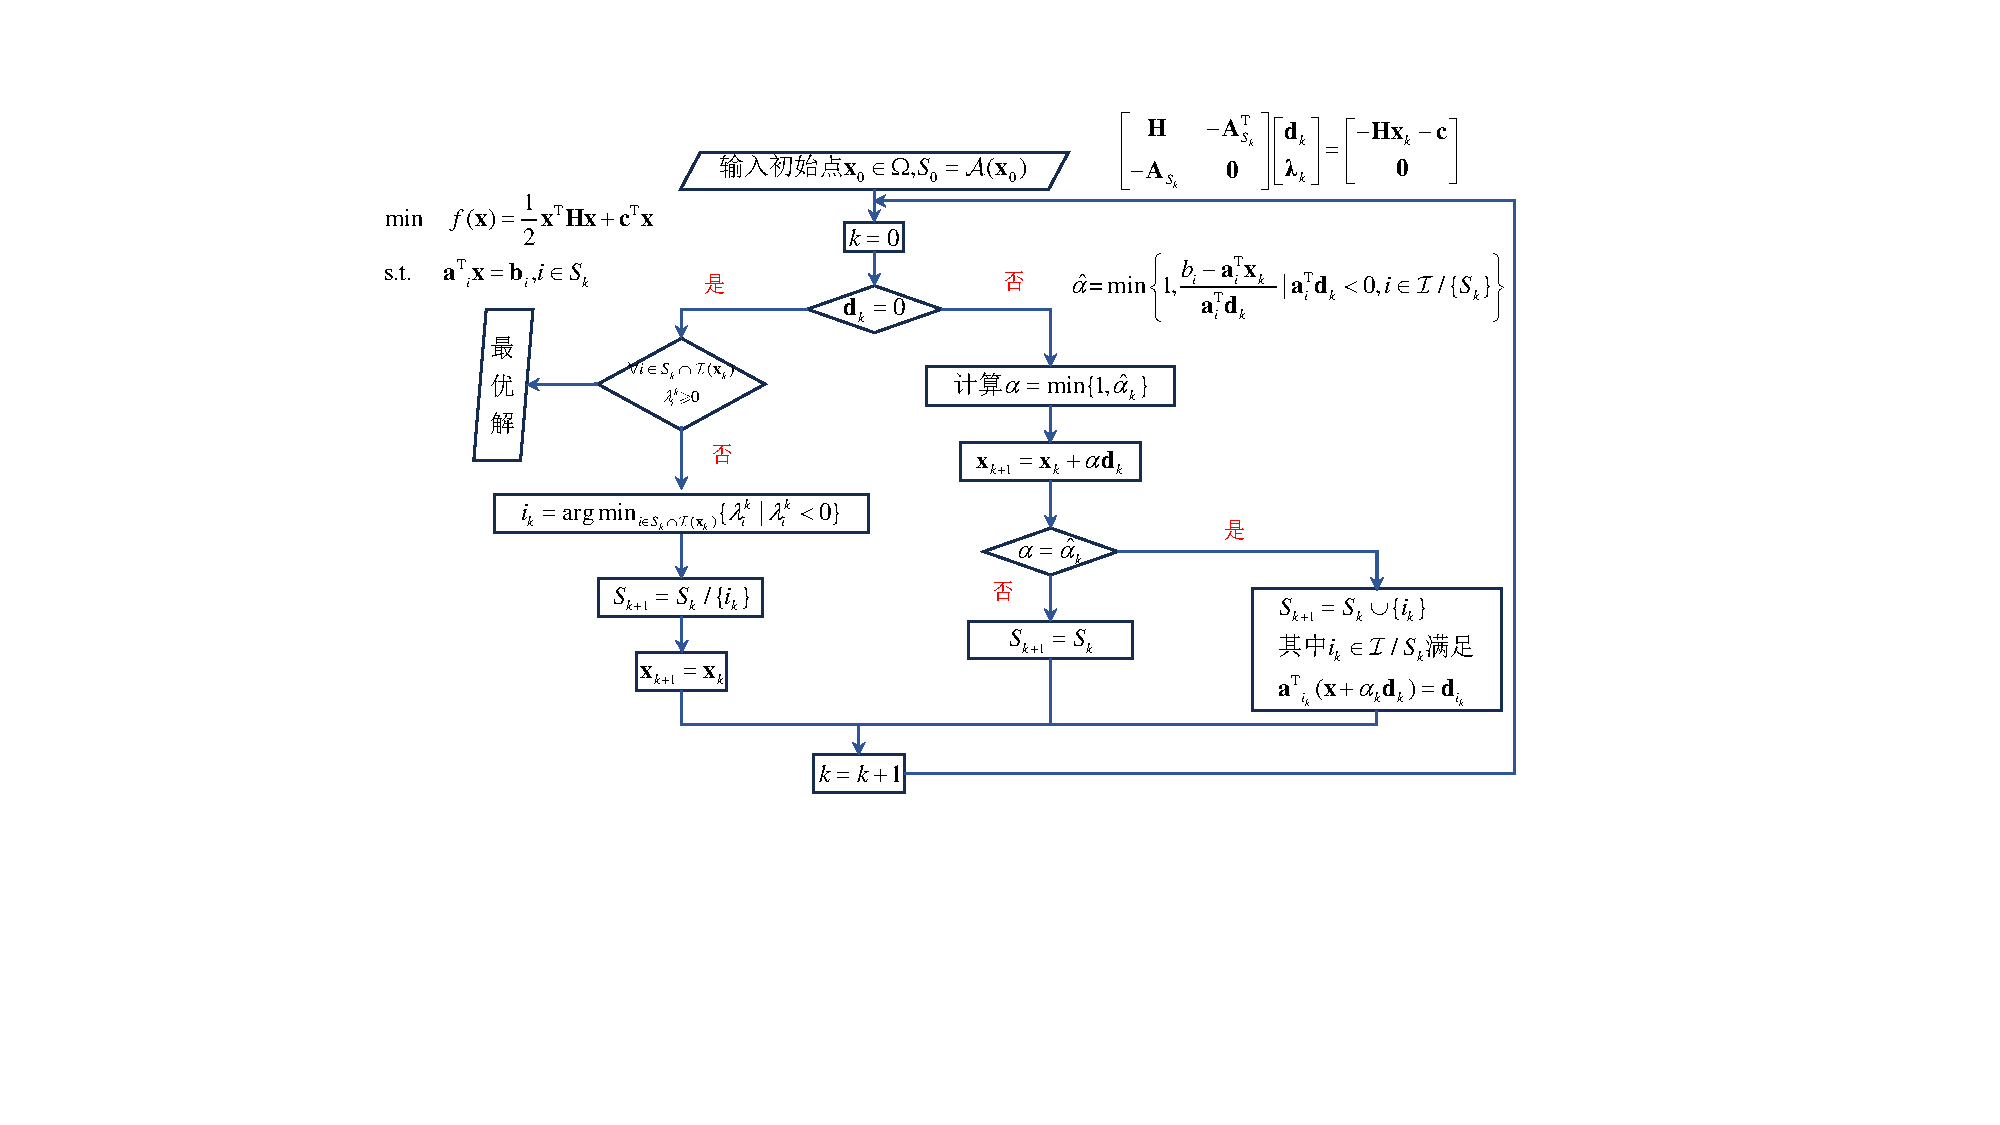
\includegraphics[width = .8\textwidth]{image/active_set-flow.pdf}
\end{figure}

\subsection{约束优化可行方向法}
\subsubsection{Zoutendijk可行方向法}
策略: 在可行条件下,让下降性达到最大

Frank-Wolfe方法:
\[
    \begin{aligned}
        \min&\nabla f(\boldsymbol{x}_k)^\mathrm{T}(\boldsymbol{x}-\boldsymbol{x}_k)\\
        \mathrm{s.t.}&\boldsymbol{x}\in\Omega
    \end{aligned}
\]
缺陷:会产生模很大,下降性很差的搜索方向

Zoutendijk可行方向法:在可行方向锥中寻求最靠近负梯度方向的搜索方向 

\[
    \boldsymbol{x}_{k}\in\Omega\Rightarrow
    \left\{
        \begin{array}{ll}
            \boldsymbol{a}_i^\mathrm{T}\boldsymbol{x}_k=b_i,&i\in\mathcal{E}\\
            \boldsymbol{a}_i^\mathrm{T}\boldsymbol{x}_k=b_i,&i\in\mathcal{I}(\boldsymbol{x}_k)\\
            \boldsymbol{a}_i^\mathrm{T}\boldsymbol{x}_k>b_i,&i\in\mathcal{I}/\mathcal{I}(\boldsymbol{x}_k)
        \end{array}
    \right. 
\]

\[
    \boldsymbol{d}_{k}\text{可行}\Rightarrow
    \begin{aligned}
        &\left\{
            \begin{array}{ll}
                \boldsymbol{a}_{i}^{\mathrm{T}}(\boldsymbol{x}_{k}+\alpha\boldsymbol{d}_{k})=b_{i},&i\in\mathcal{E}\\
                \boldsymbol{a}_{i}^{\mathrm{T}}(\boldsymbol{x}_{k}+\alpha\boldsymbol{d}_{k})\geqslant b_{i},&i\in\mathcal{I}
            \end{array}
            \right.\\
            &\left\{
                \begin{array}{ll}
                    \boldsymbol{a}_{i}^{\mathrm{T}}\boldsymbol{d}_{k}=0,&i\in\mathcal{E}\\
                    \boldsymbol{a}_{i}^{\mathrm{T}}\boldsymbol{d}_{k}\geqslant0,&i\in\mathcal{I}(\boldsymbol{x}_{k})
                \end{array}
                \right.
    \end{aligned}
\]

\[
    \begin{aligned}
        \boldsymbol{d}_{k}=\arg\min &\, d^{\mathrm{T}}\nabla f(x_{k})  \\
        \mathrm{s.t.}&\, \boldsymbol{a}_i^\mathrm{T}\boldsymbol{d}\geqslant0,\quad i\in\mathcal{I}(\boldsymbol{x}_k)  \\
        &\,\boldsymbol{a}_{i}^{\mathrm{T}}\boldsymbol{d}=0,\quad i\in\mathcal{E} \\
        &\,-1\leqslant d_{i}\leqslant1,\quad1\leqslant i\leqslant n
    \end{aligned}
\]
计算最大可行步长
\[
    \boldsymbol{a}_{i}^{\mathrm{T}}(\boldsymbol{x}_{k}+\alpha \boldsymbol{d}_{k})\geqslant b_{i},\quad\alpha\geq0,i\in\mathcal{I}/\mathcal{I}(\boldsymbol{x}_{k}^{*})
\]
\[
    \hat{\alpha}_k=\min_{i\in\mathcal{I}\setminus\mathcal{I}(\boldsymbol{x})}\left\{\frac{b_i-\boldsymbol{a}_i^\mathrm{T}\boldsymbol{x}_k}{\boldsymbol{a}_i^\mathrm{T}\boldsymbol{d}_k}|\boldsymbol{a}_i^\mathrm{T}\boldsymbol{d}_k<0\right\}
\]
最优步长
\[
    \alpha_{k}=\arg\operatorname*{min}\{f(\boldsymbol{x}_{k}+\alpha\boldsymbol{d}_{k})\mid0\leqslant\alpha\leqslant\hat{\alpha}_{k}\}
\]
\subsection{投影算子}
\begin{definition}[投影算子]
    设$\Omega$ 为非空闭凸集.对任意$\boldsymbol{x}\in\mathbb{R}^n$,定义
    \[
        P_\Omega(\boldsymbol{x})=\arg\min\{\|\boldsymbol{x}-\boldsymbol{y}\|\mid\boldsymbol{y}\in\Omega\},
    \]并称其为$\boldsymbol{x}$ 到$\Omega$上的投影。称 $P_\Omega(\cdot)$ 为从 $\mathbb{R}^n$ 到$\Omega$上的投影算子
\end{definition}
\begin{theorem}
    对闭凸锥$\mathcal{K}$和任意$\boldsymbol{x}\in\mathbb{R}^{n}$
    \begin{enumerate}
        \item $\langle \boldsymbol{x}- P_{\mathcal{K} }( \boldsymbol{x}) , P_{\mathcal{K} }( \boldsymbol{x}) \rangle = 0$,即 $\langle \boldsymbol{x}, P_{\mathcal{K} }( \boldsymbol{x}) \rangle = \| P_{\mathcal{K} }( \boldsymbol{x}) \| ^{2}$
        \item $\parallel \boldsymbol{x}\parallel\geqslant\parallel P_{\mathcal{K}}(\boldsymbol{x})\parallel$
    \end{enumerate}
    \begin{figure}[ht]
        \centering
        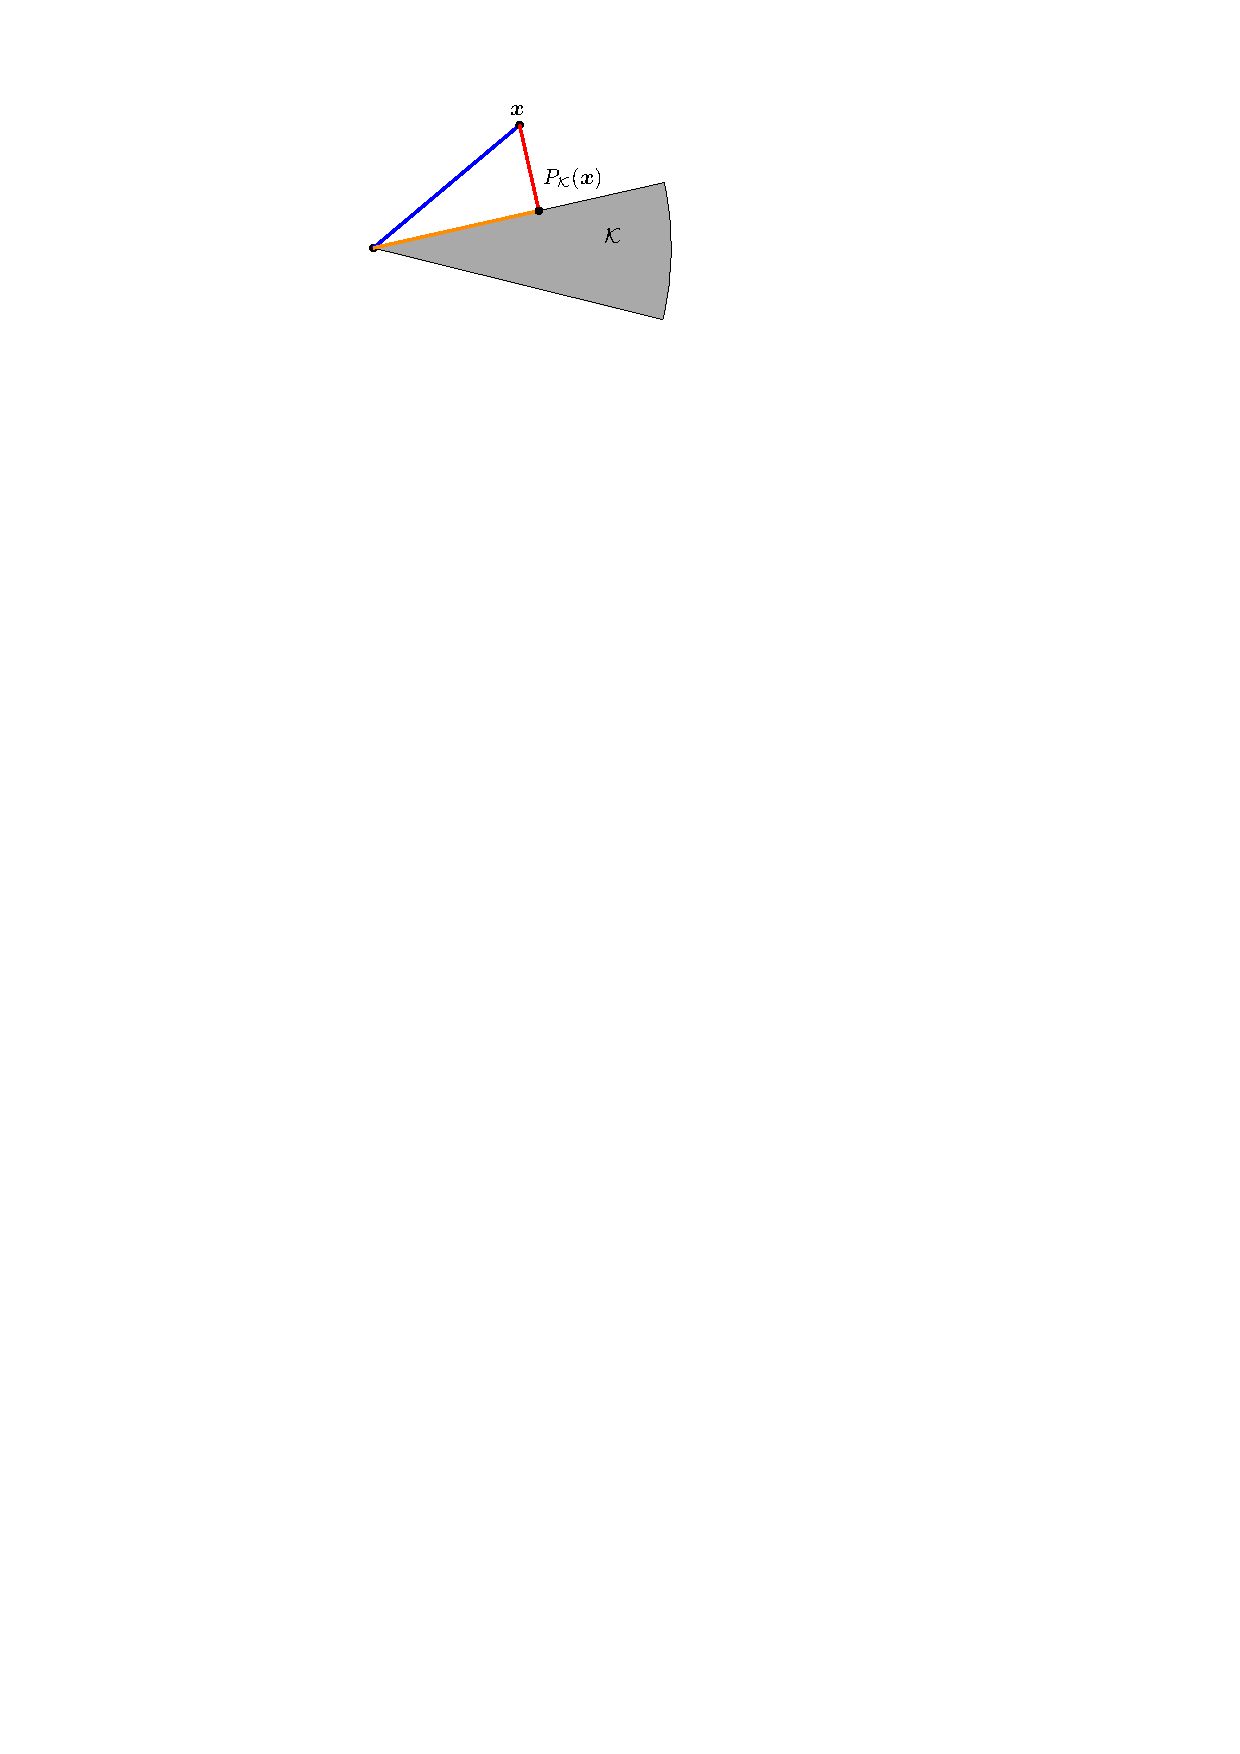
\includegraphics{image/闭凸锥上的投影.pdf}
    \end{figure}
\end{theorem}
\begin{theorem}[Moreau分解定理]
   设$\mathcal{K}$ 为非空闭凸锥,$\mathcal{K} ^0= \{ \boldsymbol{y}\in \mathbb{R} ^n\mid \langle x, \boldsymbol{y}\rangle \leqslant 0$, $\forall$ $\boldsymbol{x}\in \mathcal{K} \}$,对任意的$\boldsymbol{x}\in\mathbb{R}^n$,令 $\boldsymbol{y}= P_{\mathcal{K} }( \boldsymbol{x})$, $\boldsymbol{z}= P_{\mathcal{K} ^{\circ }}( \boldsymbol{x})$,则$\boldsymbol{x}=\boldsymbol{y}+\boldsymbol{z}$且$\langle \boldsymbol{y},\boldsymbol{z}\rangle=0.$

   \colorbox{red!50}{几何解释:任一向量可分解成闭凸锥与其极锥上的两个投影的直和。}
   \begin{figure}[ht]
        \centering
        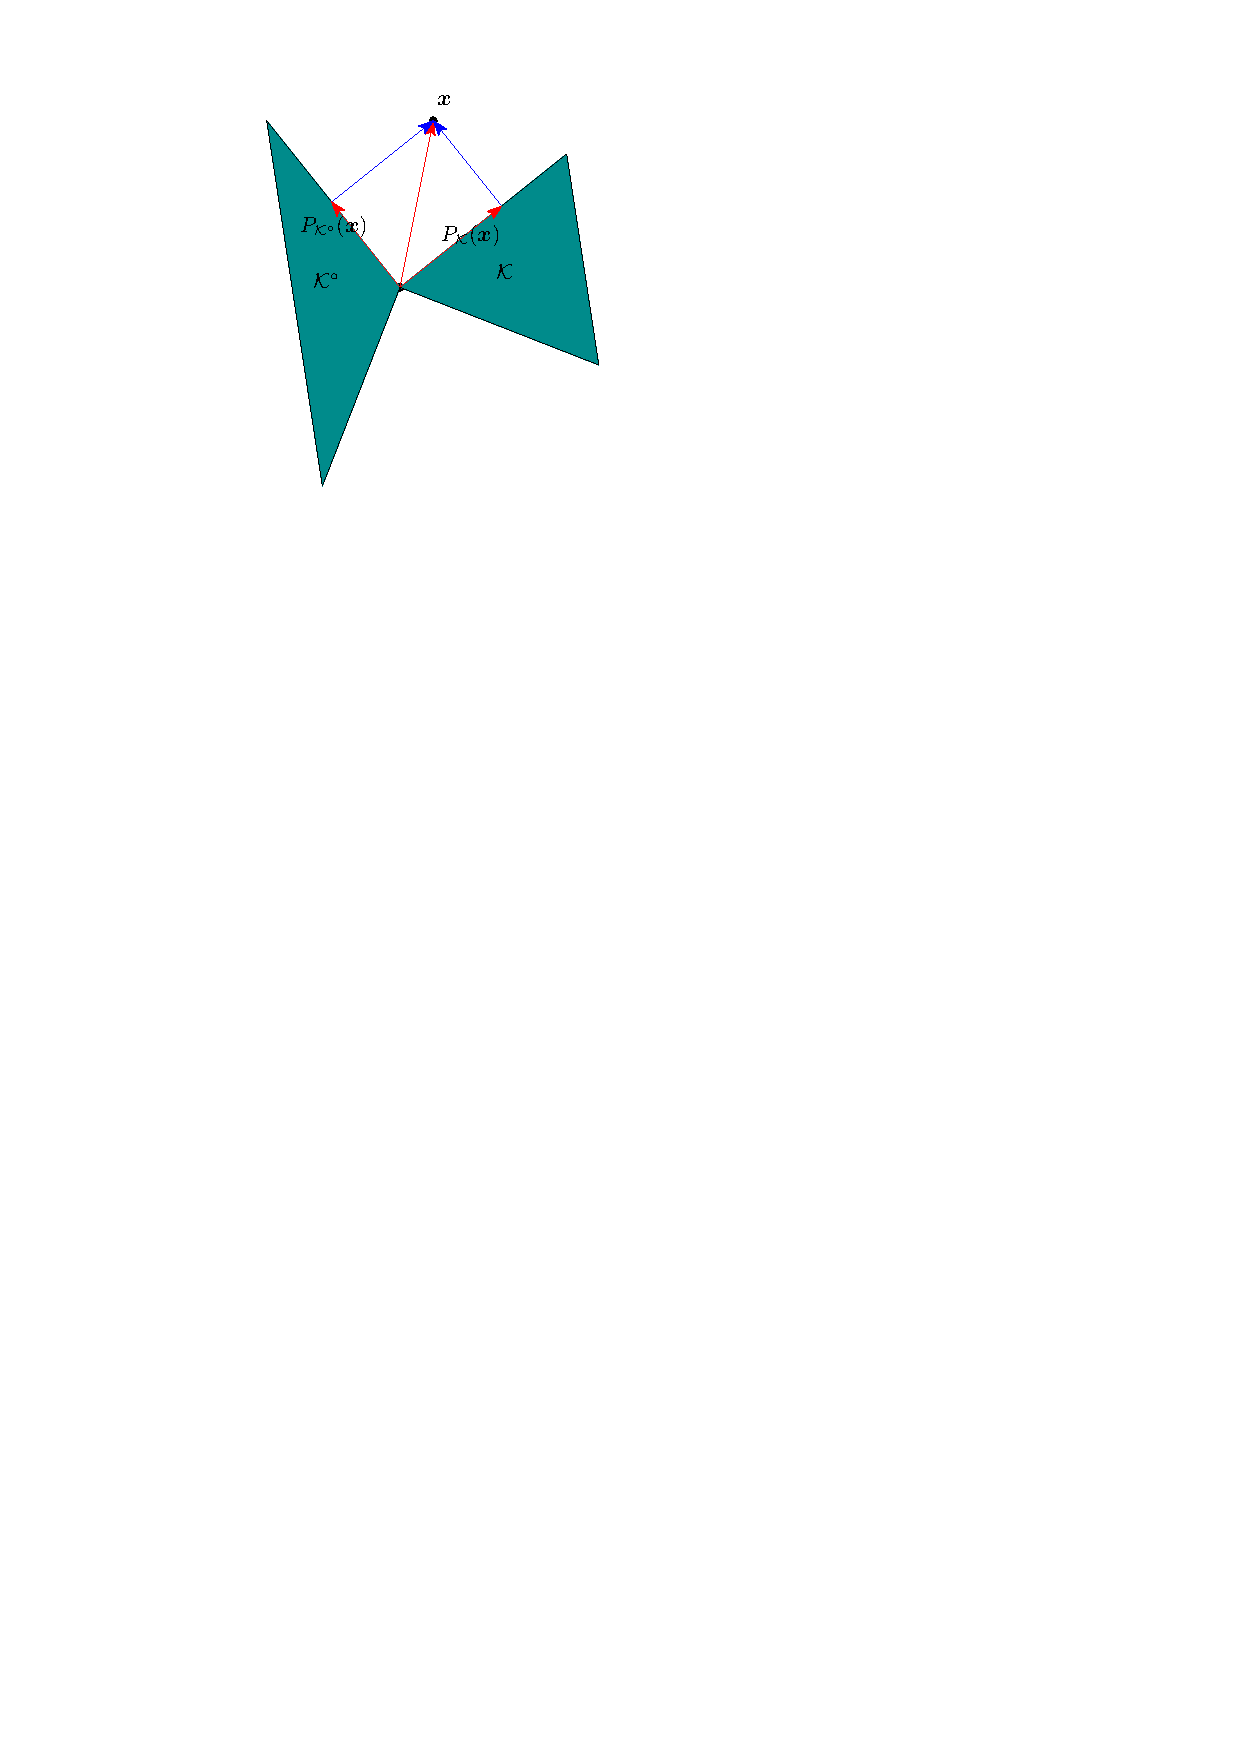
\includegraphics{image/闭凸锥上的投影分解.pdf}
   \end{figure}
\end{theorem}
\begin{theorem}
    $\boldsymbol{x}\in \Omega$ 为凸约束优化问题$\min\{f(\boldsymbol{x})\mid x\in\Omega\}$ 的稳定点,则对任意的$\alpha>0$, 均有 $\boldsymbol{x}=P_\Omega(\boldsymbol{x}-\alpha\nabla f(\boldsymbol{x}))$
    
    \textcolor{red!80}{残量函数$r(x)=\boldsymbol{x}-P_\Omega(\boldsymbol{x}-\nabla_f(\boldsymbol{x}))$可作为价值函数度量当前点与最优解(稳定点)之间的近似程度}

    \textcolor{cyan!80}{易操作的最优解判定方式。可作为算法终止规则。}
\end{theorem}
\begin{definition}
    $\boldsymbol{x}\in \Omega .$称$\mathcal{T}_\Omega(\boldsymbol{x})=\{\boldsymbol{d}\in\mathbb{R}^n\parallel\text{存在}\boldsymbol{d}_k\to \boldsymbol{d},t_k\to0^+$,使得$\boldsymbol{ x}+t_k\boldsymbol{ d}_k\in\Omega\}$为闭凸集$\Omega$在$\boldsymbol{x}$点的切锥。
\end{definition}
\begin{definition}
    定义$-\nabla f(x)$在切锥$\mathcal{T}_\Omega(x)$上的投影定义为约束优化 问题$\min \{ f( \boldsymbol{x}) \mid \boldsymbol{x}\in \Omega \}$ 在 $\boldsymbol{x}$点的投影梯度,即
    \[
        \nabla _{\Omega }f( \boldsymbol{x}) \triangleq \arg \min \{ \| \boldsymbol{d}+ \nabla f( \boldsymbol{x}) \| \mid \boldsymbol{d}\in \mathcal{T} _{\Omega }( \boldsymbol{x})\}
    \]
\end{definition}
\begin{theorem}
    $\boldsymbol{x}\in \Omega$为 约 束 优 化 问 题 $\min \{ f( \boldsymbol{x}) \mid \boldsymbol{x}\in \Omega \}$稳 定 点  当 且 仅 当 $\nabla _\Omega f( \boldsymbol{x}) = \mathbf{0} .$

    \textcolor{red!80}{几何意义:在最优值点(稳定点),负梯度属于该点的法锥。}
    \begin{figure}[H]
        \centering
        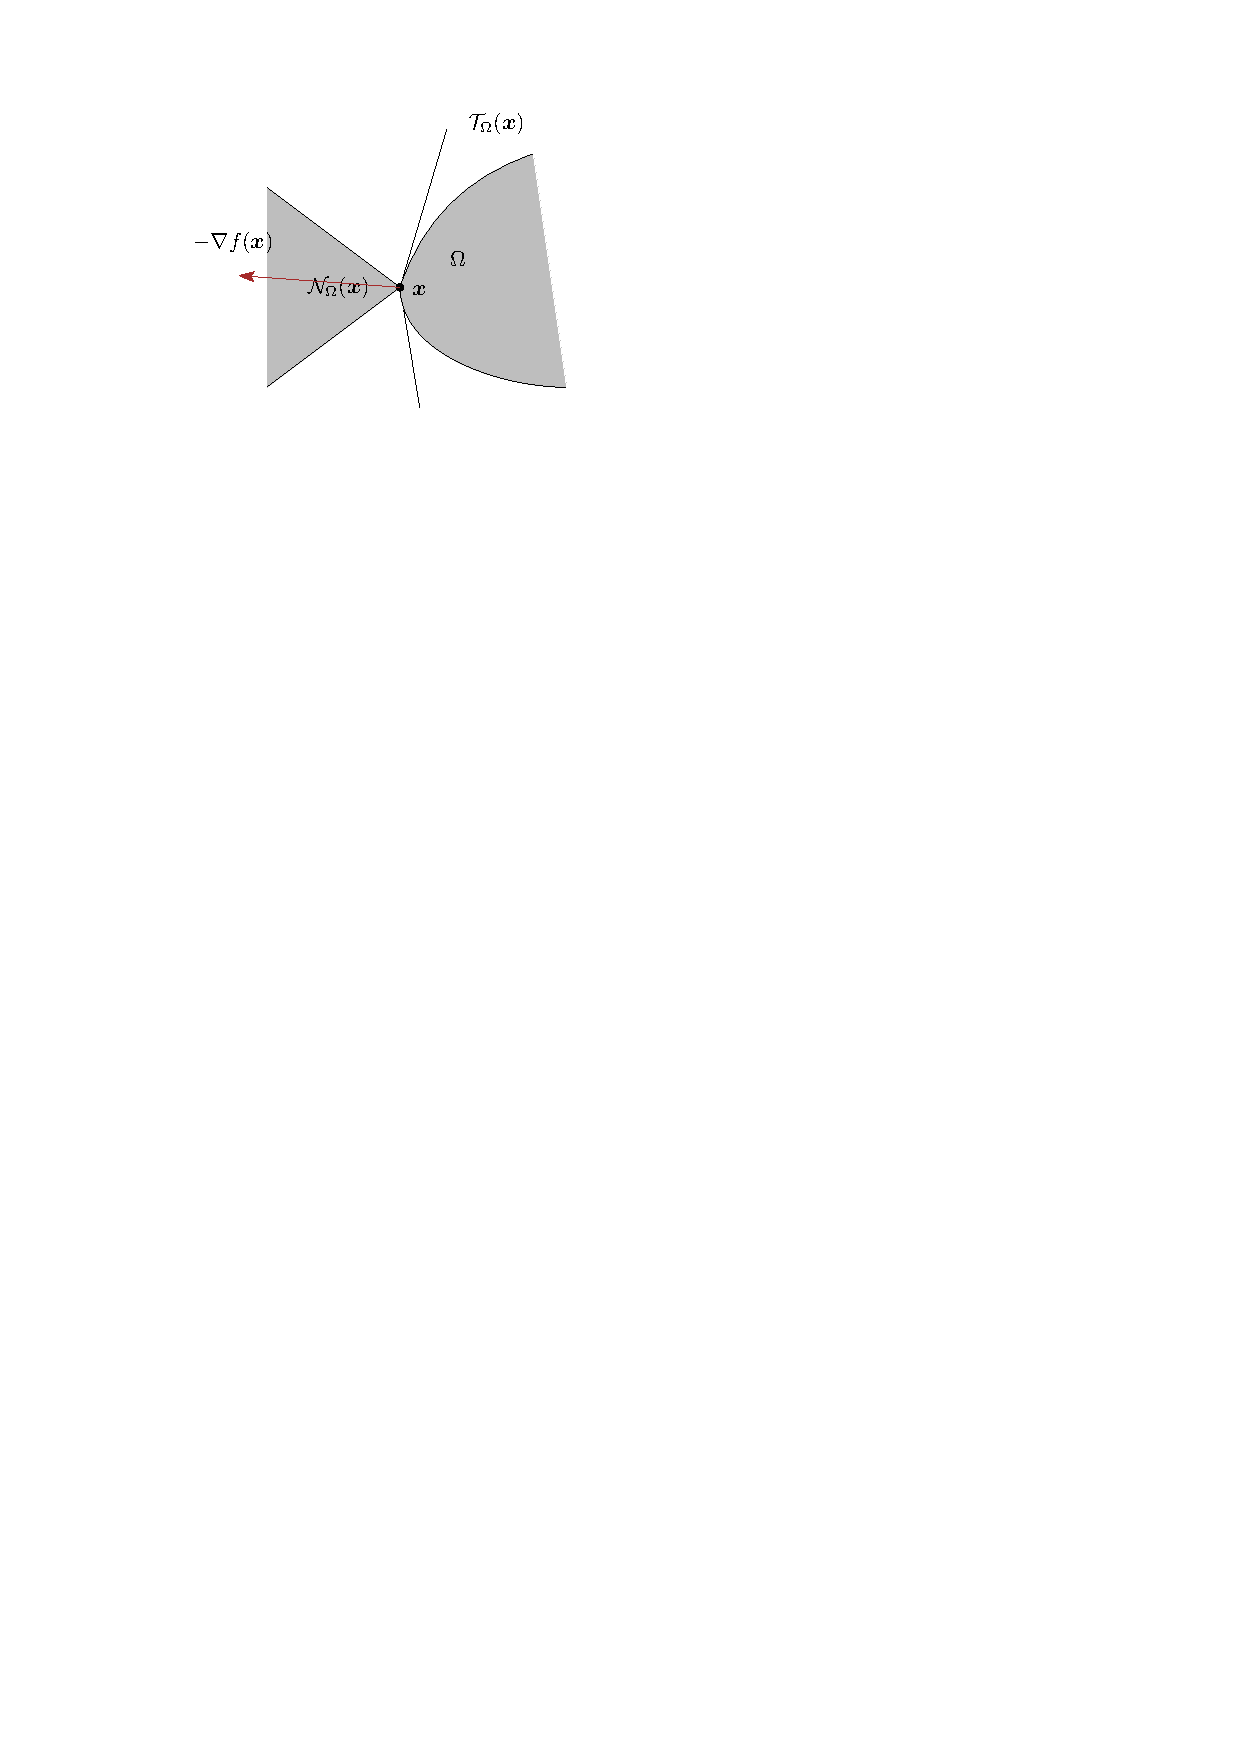
\includegraphics{image/负梯度投影.pdf}
    \end{figure}
\end{theorem}
\subsubsection{矩阵的广义逆}
若矩阵$\boldsymbol{A}$ 奇异,或者非方阵,是否存在与逆矩阵类似的矩阵?
\begin{definition}
    矩阵的广义逆:$\boldsymbol{A}\in\mathbb{R}^{m\times n}$。若存在矩阵$\boldsymbol{G}\in\mathbb{R}^{n\times m}$ 使得
    \[
        \begin{aligned}
            \boldsymbol{AGA}&=\boldsymbol{A},\quad \boldsymbol{GAG}=\boldsymbol{G},\\
            (\boldsymbol{AG})^{\mathrm{T}}&=\boldsymbol{AG},\quad(\boldsymbol{GA})^{\mathrm{T}}=\boldsymbol{GA}
        \end{aligned}
    \]
    则称矩阵$\boldsymbol{G}$为矩阵$\boldsymbol{A}$的广义逆,又称Moore-Penrose广义逆。记为$\boldsymbol{A}^+$
\end{definition}
\begin{itemize}
    \item 矩阵非奇异$\boldsymbol{A}^{+} = \boldsymbol{A}^{-1}$
    \item 矩阵行满秩$\boldsymbol{A}^{+} = \boldsymbol{A}^{\mathrm{T}}(\boldsymbol{A}\boldsymbol{A}^{\mathrm{T}})^{-1}$
    \[
        \boldsymbol{A}\colorbox{cyan!80}{$\boldsymbol{A}^{\mathrm{T}}(\boldsymbol{A}\boldsymbol{A}^{\mathrm{T}})^{-1}$}\boldsymbol{A} = \boldsymbol{A}
    \]
    \item 矩阵列满秩$\boldsymbol{A}^{+} = (\boldsymbol{A}^{\mathrm{T}}\boldsymbol{A})^{-1}\boldsymbol{A}^{\mathrm{T}}$
    \[
        \boldsymbol{A}\colorbox{cyan!80}{$(\boldsymbol{A}^{\mathrm{T}}\boldsymbol{A})^{-1}\boldsymbol{A}^{\mathrm{T}}$}\boldsymbol{A} = \boldsymbol{A}
    \]
    \item 矩阵行(或列)单位正交,即满足矩阵$\boldsymbol{A}\boldsymbol{A}^{\mathrm{T}} = \boldsymbol{I}_{m}$或者($\boldsymbol{A}^{\mathrm{T}}\boldsymbol{A} = \boldsymbol{I}_{n}$),则$\boldsymbol{A}^+ = \boldsymbol{A}^{\mathrm{T}}$
    \[  
        \boldsymbol{A} = \begin{bmatrix}
            \boldsymbol{v}_{1}^{\mathrm{T}} & \boldsymbol{v}_{2}^{\mathrm{T}} & \cdots & \boldsymbol{v}_m^{\mathrm{T}}
        \end{bmatrix}^{\mathrm{T}}\ \text{且}\ \boldsymbol{v}_{i}^{\mathrm{T}}\boldsymbol{v}_{j} = \delta_{ij}
    \]
    \[
        \boldsymbol{A}\boldsymbol{A}^{\mathrm{T}} = \begin{bmatrix}
            \boldsymbol{v}_{i}^{\mathrm{T}}\boldsymbol{v}_{j}
        \end{bmatrix}_{m\times m} = \boldsymbol{I}_{m\times m}
    \]
    有
    \[
        \boldsymbol{A}\colorbox{cyan!80}{$\boldsymbol{A}^{\mathrm{T}}$}\boldsymbol{A} = \boldsymbol{I}_{m\times m}\boldsymbol{A} = \boldsymbol{A}
    \]
\end{itemize}

\subsection{约束优化投影算法}
凸约束优化 $\min\{f(\boldsymbol{x})\mid \boldsymbol{x}\in\Omega\}$
可行域非空闭凸

基本思想:沿负梯度方向行进,借助投影算子拉回可行域

迭代格式 $\boldsymbol{x}_{k+ 1}= P_{\Omega }( \boldsymbol{x}_{k}- {\alpha } _{k}\nabla f( \boldsymbol{x}_{k}) ) .$